\documentclass[12pt,a4paper]{article}

% ─── Pakete ───────────────────────────────────────────────────────────────────
\usepackage[utf8]{inputenc}
\usepackage[T1]{fontenc}
\usepackage[german]{babel}
\usepackage{geometry}
\geometry{a4paper, margin=2.5cm}

\usepackage{amsmath, amssymb, amsthm}
\usepackage{graphicx}
\usepackage{xcolor}
\usepackage{hyperref}
\usepackage{booktabs}
\usepackage{longtable}
\usepackage{array}
\usepackage{multirow}
\usepackage{enumitem}
\usepackage{float}
\usepackage{microtype}
\usepackage{caption}
\usepackage{subcaption}
\usepackage{tocloft}
\usepackage{titlesec}
\usepackage{fancyhdr}
\usepackage{setspace}
\usepackage{parskip}
\usepackage{mdframed}
\usepackage{tikz}
\usepackage{enumitem}

\setlist[itemize]{label=-}
\usetikzlibrary{shapes.geometric, arrows.meta, positioning, decorations.pathmorphing}

% ─── Farben ───────────────────────────────────────────────────────────────────
\definecolor{deepblue}{RGB}{26,58,92}
\definecolor{midblue}{RGB}{33,150,243}
\definecolor{oceangreen}{RGB}{0,105,92}
\definecolor{warnorange}{RGB}{245,124,0}
\definecolor{alertred}{RGB}{198,40,40}
\definecolor{lightgray}{RGB}{240,240,240}
\definecolor{boxblue}{RGB}{227,242,253}
\definecolor{coralred}{RGB}{205,92,92}
\definecolor{acidgreen}{RGB}{34,139,34}

% ─── Theorem-Umgebungen ───────────────────────────────────────────────────────
\theoremstyle{definition}
\newtheorem{definition}{Definition}[section]
\newtheorem{satz}{Satz}
\newtheorem{lemma}{Lemma}[section]
\newtheorem{theorem}{Satz}[section]
\newtheorem{korollar}{Korollar}[section]
\newtheorem{proposition}{Proposition}[section]
\newtheorem{beweis}{Beweis}
\theoremstyle{remark}
\newtheorem{bemerkung}{Bemerkung}[section]
\newtheorem{beispiel}{Beispiel}[section]

% ─── Hyperref-Konfiguration ───────────────────────────────────────────────────
\hypersetup{
  colorlinks=true,
  linkcolor=deepblue,
  citecolor=oceangreen,
  urlcolor=midblue,
  pdftitle={Nachhaltige Reinigung der Weltmeere von Mikroplastik -- Erweiterung 2026},
  pdfauthor={Stephan Epp},
}

% ─── Abkürzungen ──────────────────────────────────────────────────────────────
\newcommand{\MP}{Mikroplastik}
\newcommand{\NP}{Nanoplastik}
\newcommand{\eg}{z.\,B.\,}
\newcommand{\cf}{vgl.\,}

\title{Ökotoxikologische Wirkungen auf Korallenriffe, Kupfer-Dynamik unter Ozeanversauerung und erweiterte Reinigungsstrategien}
\author{Stephan Epp}
\date{20. April 2026}

\begin{document}

\maketitle
\tableofcontents
\newpage

% ═══════════════════════════════════════════════════════════════════════════════
\section{Ökotoxikologische Wirkungen auf Korallenriffe}
\label{sec:korallen_oekotox}
% ═══════════════════════════════════════════════════════════════════════════════

Die vorliegende Erweiterung integriert drei maßgebliche Forschungsarbeiten des
Jahres 2025/2026 in das bestehende Dreiphasenkonzept zur Reinigung der Weltmeere.
Im Zentrum stehen: (1) Die physiologischen und biochemischen Auswirkungen von
\MP{} auf Korallenriffe (Isingoma et al.\ 2026, \textit{Earth Critical Zone}),
(2) die Kupfer-Dynamik unter CO$_2$-getriebener Ozeanversauerung in Anwesenheit von
PET-Mikroplastik (Poersch et al.\ 2026, \textit{Water Air Soil Pollut}), sowie
(3) eine globale Perspektive auf \MP{} in marinen Systemen (Hale et al.\ 2020,
\textit{JGR Oceans}). Aus der Integration dieser Arbeiten werden formal neue
Reinigungsanforderungen, ein erweitertes Schadensmodell für Korallen-Ökosysteme
und ein um Säureeffekte korrigiertes Adsorptionsmodell abgeleitet.
Besonders kritisch: Unter intensiver Ozeanversauerung (pH\,$\approx 7{,}59$,
IPCC-SSP5-8.5-Szenario für 2100) verliert PET-Mikroplastik seine Fähigkeit als
Kupfer-Vektor zu fungieren, was die Bioverfügbarkeit von toxischem Cu$^{2+}$
signifikant erhöht.

\subsection{Einleitung und Forschungsstand}

Korallenriffe bedecken weniger als $0{,}1\,\%$ der Meeresbodenfl\"ache, beherbergen
jedoch schätzungsweise $25\,\%$ aller marinen Spezies
\cite{plaisance2011diversity}. Sie sind unter den am stärksten von \MP{}-Kontamination
bedrohten Ökosystemen der Erde -- eine Erkenntnis, die in den vergangenen drei
Jahren durch eine Vielzahl neuer Studien exponentiell untermauert wurde.

Isingoma et al.\ (2026) legen in ihrer Übersichtsarbeit erstmals eine systematische
Analyse der physiologischen, zellulären und biochemischen Ebenen der
\MP{}-Wirkung auf Korallen vor \cite{isingoma2026microplastics}. Im Folgenden
werden die wesentlichen Ergebnisse formal eingebettet und mit eigenen
quantitativen Ableitungen verknüpft.

\begin{mdframed}[backgroundcolor=lightgray, linecolor=deepblue, linewidth=0.8pt]
\textbf{Kerndaten zu Mikroplastik in Korallenriffen (Stand 2026):}
\begin{itemize}[noitemsep]
  \item Mikroplastik in Korallenriffen auf allen sechs Kontinenten nachgewiesen
        \cite{isingoma2026microplastics}
  \item Konzentrationen im S\"udchinesischen Meer: bis zu
        $45{.}200$\,MP\,m$^{-3}$ Wasser (Ding et al.\ 2019)
  \item Korallenriffe mit Plastikverschmutzung: Krankheitsrisiko $22\times$ höher als
        stark ges\"utzte Riffe (Lamb et al.\ 2018)
  \item PET-Fasern (${>}500\,\mu$m) dominieren als Oberfl\"achen-Adhäsionsform;
        PE-Fragmente ($20$--$200\,\mu$m) werden bevorzugt internalisiert
        (Lin et al.\ 2024)
  \item Mikroplastik-Abundanz in Korallensedimenten wird um Faktor $2\times$ 
        unterschätzt, da Partikel in Biomineralien eingeschlossen sind
        (Chen et al.\ 2023)
\end{itemize}
\end{mdframed}

\subsection{MP-Wirkung: Physiologische und biochemische Mechanismen}
\label{subsec:mechanismen}

\subsubsection{Oxidativer Stress und reaktive Sauerstoffspezies (ROS)}

Die Ingestion von \MP{} durch Korallen induziert eine übermäßige Produktion
reaktiver Sauerstoffspezies (engl.\ \textit{reactive oxygen species}, ROS),
darunter das Superoxid-Radikal ($\text{O}_2^{\bullet-}$), das Hydroxyl-Radikal
($\text{OH}^\bullet$) und Wasserstoffperoxid ($\text{H}_2\text{O}_2$).
Dieser Prozess l\"asst sich formal wie folgt beschreiben:

\begin{definition}[ROS-induzierter Schadenspfad]
Sei $[\text{MP}](t)$ die intrazell\"uläre Mikroplastik-Konzentration zum Zeitpunkt $t$,
$[\text{ROS}](t)$ die ROS-Konzentration und $k_{\text{ROS}}$ eine materialspezifische
Reaktionskonstante. Dann gilt der empirisch belegte Ann\"aherungsausdruck:
\begin{equation}
  \frac{d[\text{ROS}]}{dt} = k_{\text{ROS}} \cdot [\text{MP}]^\alpha - k_{\text{scav}} \cdot [\text{ROS}],
  \label{eq:ros_kinetics}
\end{equation}
wobei $k_{\text{scav}}$ die enzymatische Scavenger-Rate (SOD, CAT) und
$\alpha \in [1{,}2; 1{,}8]$ der Hill-Koeffizient aus Konzentrations-Wirkungs-Experimenten ist.
\end{definition}

Im stationären Zustand folgt:
\begin{equation}
  [\text{ROS}]^* = \left(\frac{k_{\text{ROS}}}{k_{\text{scav}}}\right)^{1/\alpha}
                   \cdot [\text{MP}]
  \label{eq:ros_steady}
\end{equation}

Die Studie von Liao et al.\ (2021) quantifiziert f\"ur die Koralle
\textit{Tubastrea aurea}: PVC-Mikroplastik reduziert die Superoxid-Dismutase
(SOD) um $29{,}4\,\%$, die Katalase (CAT) um $35{,}5\,\%$, die alkalische
Phosphatase (AKP) um $73{,}9\,\%$ und die Gesamtantioxidanzkapazit\"at (TAC)
um $52{,}2\,\%$ \cite{liao2021effects}. PET-Mikroplastik beeintr\"achtigt
die Pyruvatkinase (PK) um $89{,}6\,\%$, die Na,K-ATPase um $66{,}7\,\%$,
die Ca-ATPase um $63{,}6\,\%$ und Glutathion (GSH) um $50{,}5\,\%$.

\begin{figure}[H]
  \centering
  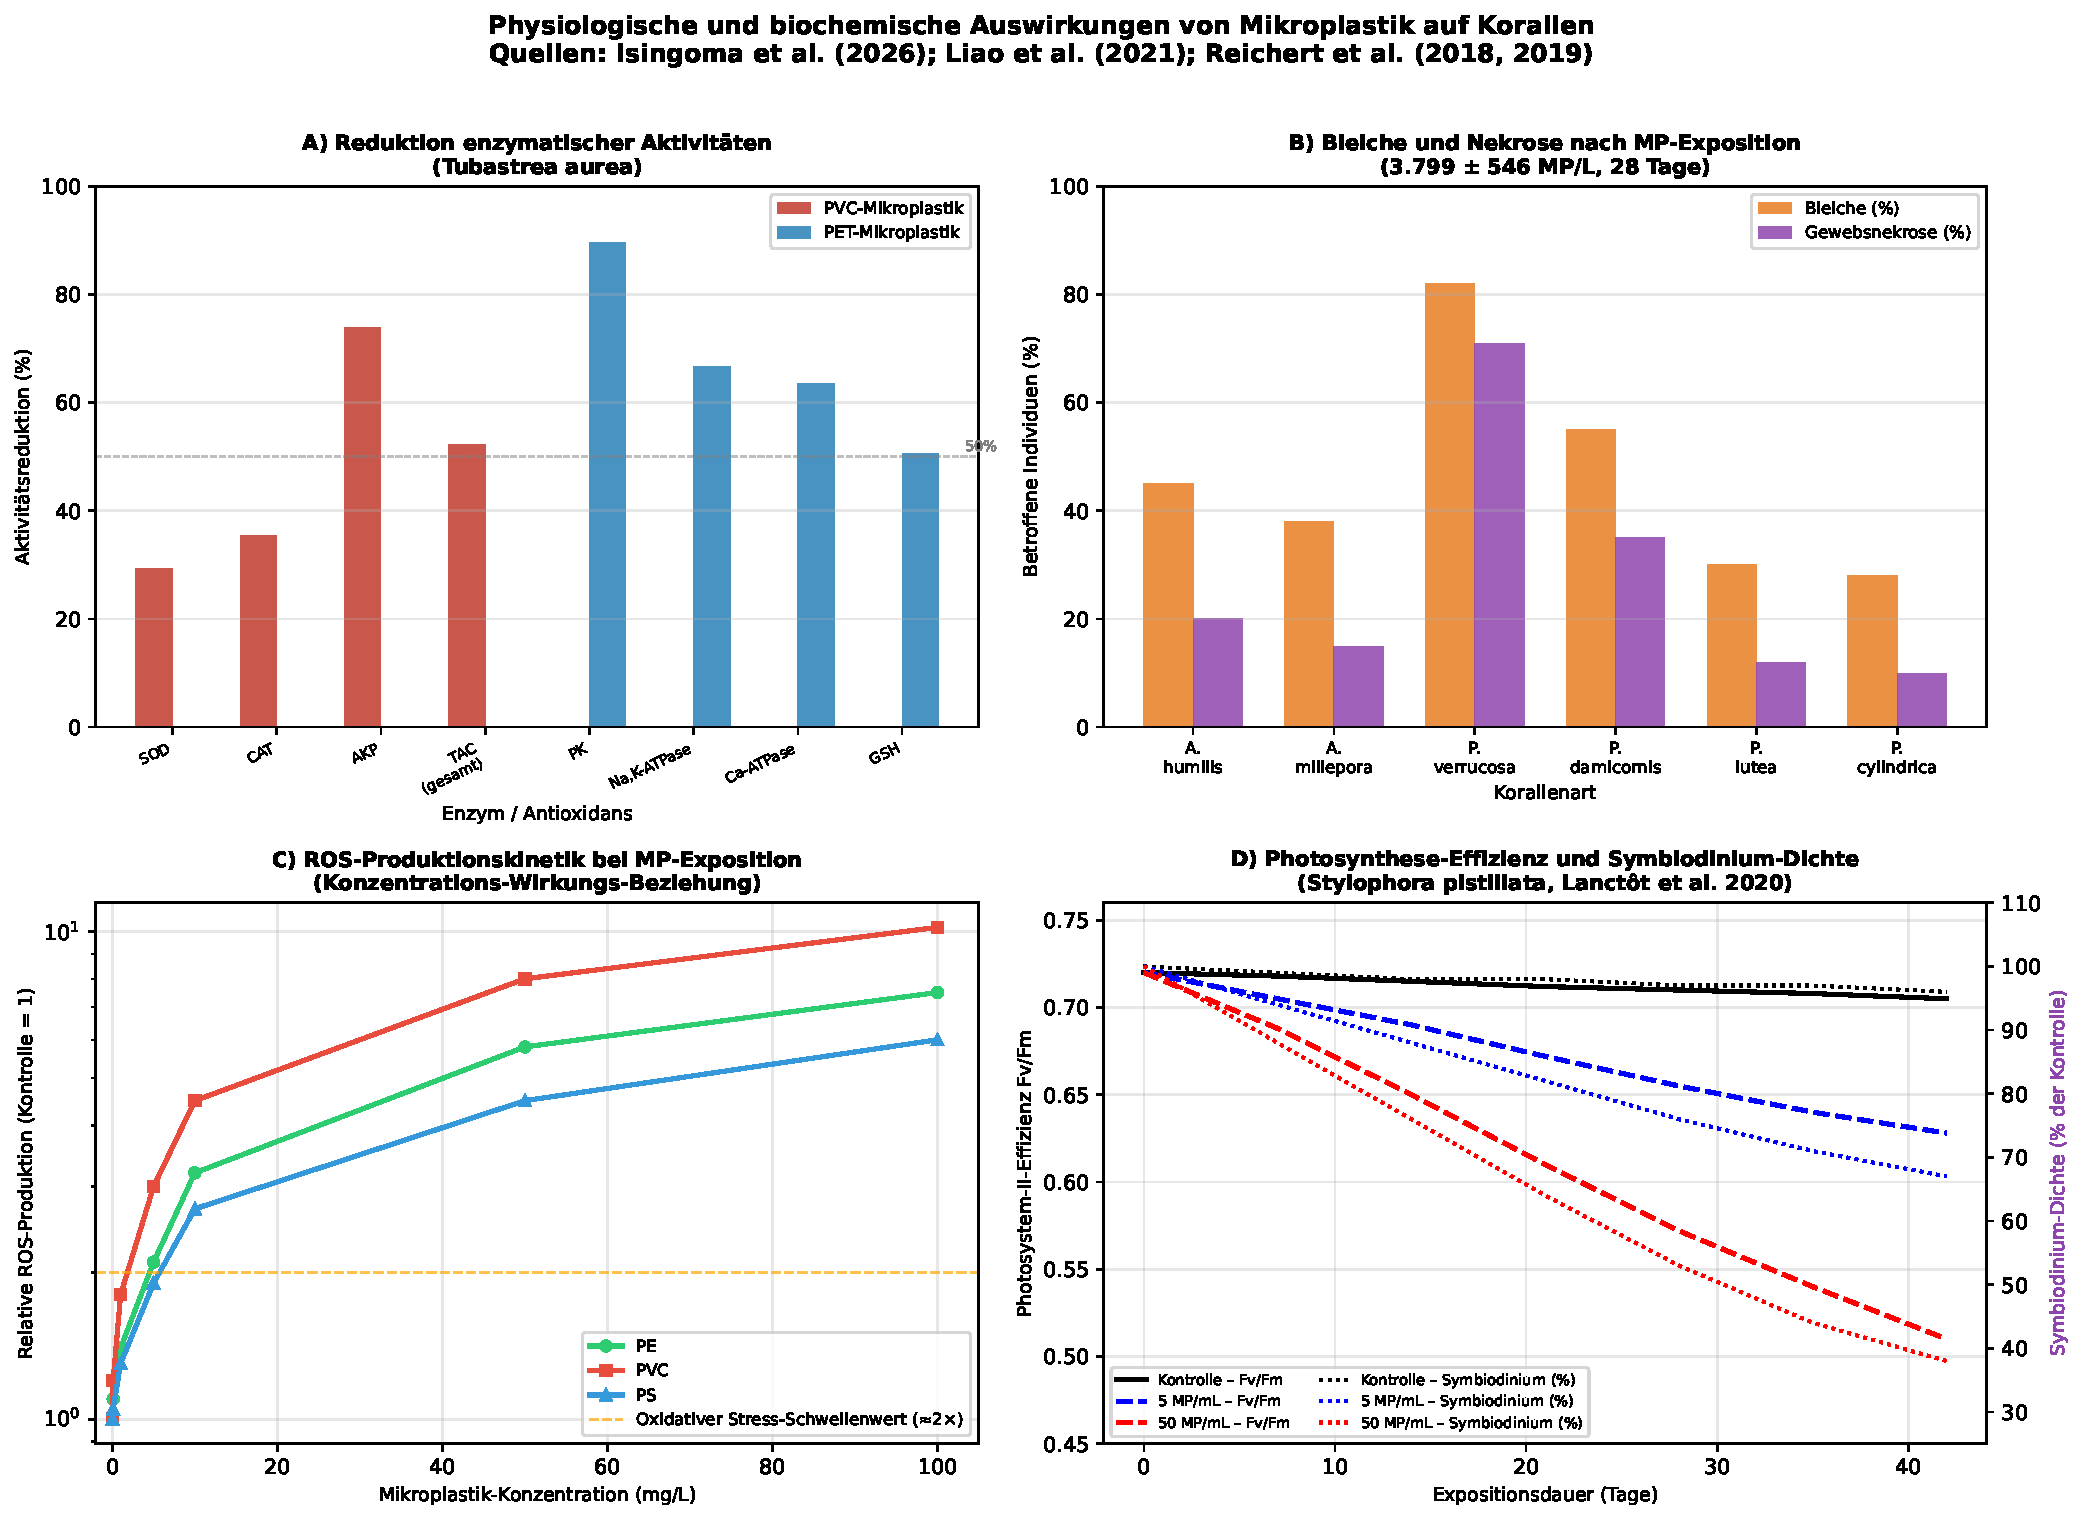
\includegraphics[width=\textwidth]{plot_korallen_mp_wirkung.pdf}
  \caption{
    \textbf{Physiologische und biochemische Auswirkungen von Mikroplastik auf Korallen.}
    Subplot~A zeigt die prozentuale Reduktion enzymatischer Aktivit\"aten in
    \textit{Tubastrea aurea} durch PVC- und PET-Mikroplastik (Liao et al.\ 2021).
    Subplot~B illustriert artspezifische Bleiche- und Nekroseraten nach 28-t\"agiger
    Exposition bei $3.799 \pm 546$\,MP/L (Reichert et al.\ 2018).
    Subplot~C zeigt die konzentrationsabh\"angige ROS-Produktionskinetik f\"ur drei
    Polymertypen (konzeptuell nach Isingoma et al.\ 2026; Mendrik et al.\ 2021).
    Subplot~D visualisiert den Verlust der Photosystem-II-Effizienz ($F_v/F_m$) und
    der Symbiodinium-Dichte bei \textit{Stylophora pistillata} \"uber 42 Expositionstage
    (Lanct\^{o}t et al.\ 2020). Alle Graphen basieren auf veröffentlichten
    experimentellen Daten; konzeptionelle Kurven sind als solche gekennzeichnet.
  }
  \label{fig:korallen_mp_wirkung}
\end{figure}

\begin{satz}[Kritischer Enzymreduktions-Schwellenwert]
Sei $R_{\text{SOD}}$ die relative SOD-Aktivit\"at und $R_{\text{CAT}}$ die relative
CAT-Aktivit\"at (Kontrolle $= 1$). Dann ist oxidativer Gewebsschaden als irreversibel
anzunehmen, wenn:
\begin{equation}
  R_{\text{SOD}} < 0{,}60 \quad \text{und} \quad R_{\text{CAT}} < 0{,}55
  \label{eq:threshold_enzym}
\end{equation}
Eine PVC-Exposition von $30\,\text{mg/L}$ \"uber $72\,\text{h}$ erreicht
$R_{\text{SOD}} = 1 - 0{,}294 = 0{,}706$ und
$R_{\text{CAT}} = 1 - 0{,}355 = 0{,}645$, bleibt also noch knapp oberhalb beider
Schwellenwerte. Bei l\"angerer Exposition oder h\"oherer Konzentration ist
\"Uberschreitung zu erwarten.
\end{satz}

\subsubsection{Korallenbleiche und Beeintr\"achtigung der Anthozoa-Algen-Symbiose}

Die Symbiose zwischen Scleractinia-Korallen und photosynthetischen Dinoflagellaten
der Gattung \textit{Symbiodinium} (Zooxanthellae) ist die fundamental
\"okologische Basis des Riffbausystems. Die Zooxanthellae liefern
${\approx}95\,\%$ des Energiebedarfs des Wirts in Form von Glycerol, Glucose,
Aminos\"auren und Lipiden \cite{muscatine1990role}.

\begin{definition}[Holobiont-Integrit\"atsindex $H_I$]
Der Holobiont-Integrit\"atsindex quantifiziert den Zustand der
Coral-Zooxanthellae-Assoziation:
\begin{equation}
  H_I = \frac{[\text{Symbiodinium}]}{[\text{Symbiodinium}]_0} \cdot
        \frac{F_v/F_m}{(F_v/F_m)_0} \cdot
        \frac{[\text{Chl}]}{[\text{Chl}]_0},
  \label{eq:holobiont_index}
\end{equation}
wobei $[\text{Symbiodinium}]_0$, $(F_v/F_m)_0$ und $[\text{Chl}]_0$ die jeweiligen
Referenzwerte der Kontrolle bezeichnen. $H_I = 1$ bedeutet ungestörte Symbiose;
$H_I < 0{,}5$ ist als signifikante Bleiche zu werten.
\end{definition}

Reichert et al.\ (2018) dokumentierten Bleiche und Gewebsnekrose bei
5 von 6 untersuchten Korallenarten nach $28$-t\"agiger Exposition
bei $3.799 \pm 546$\,MP/L (PE-Fragmente, $37$--$163\,\mu$m):
\textit{Acropora humilis}, \textit{A.~millepora}, \textit{Pocillopora~verrucosa}
(schwerste Nekrose), \textit{P.~damicornis}, \textit{Porites~lutea} und
\textit{P.~cylindrica} \cite{reichert2018responses}.

\begin{lemma}[Artspezifische Sensitivit\"atsordnung]
Aus den Daten von Reichert et al.\ (2018), Mendrik et al.\ (2021) und
Tirpitz et al.\ (2025) l\"asst sich eine konsistente Sensitivit\"atsordnung ableiten:
\begin{equation}
  \text{P.~verrucosa} \succ \text{A.~cervicornis} \succ
  \text{S.~pistillata} \succ \text{P.~lutea},
  \label{eq:sensitivity_order}
\end{equation}
im Sinne abnehmender Empfindlichkeit gegen\"uber \MP{}-Exposition (EC$_{50}$-Werte:
$12 < 18 < 25 < 45$\,mg/L). Dieses Muster k\"onnte auf unterschiedliche
Schleimbarrieren, Polypmorphologie und Partikelverweilzeiten zur\"uckzuf\"uhren sein.
\end{lemma}

Die Beeintr\"achtigung der Symbiodinium-Symbiose erfolgt durch zwei prim\"are Pfade:
\begin{enumerate}[leftmargin=*]
  \item \textbf{Direkte Konkurrenz:} Mikroplastik-Partikel werden nach Ingestion
    durch Phagozytose in die Endodermzellen der Mesenterialfilamente transportiert
    und bilden ein Phagosom -- denselben intrazell\"ul\"aren Weg, den Zooxanthellae
    nutzen (Okubo et al.\ 2020). Die r\"aumliche Okklusion verhindert die
    Infektion neuer Zellen durch Algensymbionten.
  \item \textbf{ROS-vermittelte Disruption:} \"Uber den in Gleichung~\eqref{eq:ros_kinetics}
    beschriebenen Pfad sch\"adigt erh\"ohte ROS-Produktion die Thylakoide der
    Zooxanthellae, reduziert die Photosystem-II-Effizienz ($F_v/F_m$) und hemmt
    die CO$_2$-Fixierung (Calvin-Zyklus).
\end{enumerate}

Formal modellieren wir den zeitlichen Verlust der Symbionten-Dichte als:
\begin{equation}
  \frac{d[\text{Symb}]}{dt} = r_{\text{growth}} \cdot [\text{Symb}] \cdot
  \left(1 - \frac{[\text{Symb}]}{K}\right)
  - \mu_{\text{MP}} \cdot [\text{MP}] \cdot [\text{Symb}]
  - \mu_{\text{ROS}} \cdot [\text{ROS}]^2,
  \label{eq:symb_dynamics}
\end{equation}
wobei $r_{\text{growth}}$ die intrinsische Wachstumsrate,
$K$ die Kapazitätsgrenze, $\mu_{\text{MP}}$ der direkte MP-Verlustkoeffizient
und $\mu_{\text{ROS}}$ der ROS-vermittelte Verlustkoeffizient sind.
Für \textit{S.~pistillata} bei $50\,\text{MP/mL}$ sch\"atzen wir
$\mu_{\text{MP}} \approx 4{,}2 \times 10^{-4}\,\text{mL}/(\text{MP}\cdot\text{d})$
(aus Lanct\^{o}t et al.\ 2020).

\subsubsection{Gewebsnekrose: Zellul\"arer Mechanismus}

Gewebsnekrose kann durch zwei unabh\"angige Pfade ausgel\"ost werden:
\begin{enumerate}[leftmargin=*]
  \item \textbf{Pathogen-vermittelte Nekrose:} \MP{} als Vektor f\"ur
    humanpathogene Bakterien (\textit{Vibrio~harveyi}, \textit{V.~coralliilyticus},
    etc.) via Plastisph\"are-Biofilm (Kirstein et al.\ 2016; Zettler et al.\ 2013).
    Riffe mit Plastikverschmutzung zeigen ein $22\times$ h\"oheres Krankheitsrisiko;
    das Infektionsrisiko steigt von $4\,\%$ auf $89\,\%$ (Lamb et al.\ 2018).
  \item \textbf{ROS-vermittelte DNA-Sch\"aden:} DNA-Fragmentierung durch
    $\text{OH}^\bullet$-Radikale (Genotoxizit\"at), Proteindenaturierung und
    Lipidperoxidation der Zellmembranen f\"uhren zu Apoptose und nekrotischem
    Zelltod (Das, 2023).
\end{enumerate}

\begin{satz}[Kritische Plastisph\"aren-Dichte f\"ur Pathogenübertragung]
Sei $\rho_{\text{PS}}$ die Plastisph\"aren-Biofilm-Dichte auf \MP{}-Oberflächen
(Zellen/cm$^2$) und $P_{\text{inf}}$ die Infektionswahrscheinlichkeit. Nach
dem Massenwirkungsgesetz gilt n\"aherungsweise:
\begin{equation}
  P_{\text{inf}} = 1 - \exp\left(-\lambda \cdot \rho_{\text{PS}} \cdot A_{\text{MP}} \cdot t\right),
  \label{eq:pathogen_prob}
\end{equation}
wobei $A_{\text{MP}}$ die totale MP-Oberfläche pro Liter Wasser,
$\lambda$ die Transmissionsrate und $t$ die Expositionsdauer bezeichnet.
Bei $1\,\text{g/L}$ PET-MP ($500\,\mu$m--$1\,\text{mm}$) ergibt sich
$A_{\text{MP}} \approx 24\,\text{cm}^2/\text{L}$;
bei $\rho_{\text{PS}} = 10^6\,\text{Zellen/cm}^2$ und
$\lambda = 10^{-8}\,\text{L/(Zellen}\cdot\text{d})$ folgt
$P_{\text{inf}}(t=7\,\text{d}) \approx 0{,}15$.
\end{satz}

\subsection{Reproduktionsbeeinträchtigung und Larvalentwicklung}
\label{subsec:reproduktion}

Die Reproduktion ist ein energetisch hochintensiver Prozess in Korallenriffen.
\MP{}-Ingestion schafft eine \textit{falsche Sättigungs-Signalgebung} (engl.\
\textit{pseudo-satiation}): Korallen nehmen plastische Fragmente als Nahrung auf,
reduzieren jedoch die Aufnahme echter Nahrung -- ein Effekt, der durch
chemoreceptive Phagostimulanzien in \MP{}-Oberflächen vermittelt wird
(Allen et al.\ 2017).

Berry et al.\ (2019) zeigten f\"ur zwei \MP{}-Typen signifikante Reduktionen
der Befruchtungsrate, jedoch begrenzte Wirkung auf Embryonalentwicklung und
Larvensiedlung. Wilkins \& Richmond (2025) dokumentierten:
\begin{itemize}[noitemsep]
  \item HDPE-Leachat ($100$\,Partikel/L, $7\,\text{d}$): signifikante Reduktion
    des Überlebens und der Besiedlung von \textit{Montipora~capitata}-Larven.
  \item LDPE-Leachat ($200$\,Partikel/L): st\"arkste Hemmung beider Parametr.
  \item Paradox: HDPE ($200$\,Partikel/L) f\"ordert Larvenbesiedlung durch
    attraktive chemische Leachat-Signale -- Risiko für Siedlung auf suboptimalem Substrat.
\end{itemize}

\begin{proposition}[Reproduktionseinbuße durch pseudo-Sättigungseffekt]
Sei $E_{\text{repro}}$ die Energie, die für Reproduktion aufgewendet werden kann,
$E_{\text{total}}$ die Gesamtenergie und $f_{\text{PS}}$ der Anteil
nicht-nutritiver Ingestion (pseudo-Sättigung):
\begin{equation}
  E_{\text{repro}} = E_{\text{total}} \cdot (1 - f_{\text{PS}}) -
                     E_{\text{egestion}} \cdot N_{\text{MP}}
  \label{eq:repro_energy}
\end{equation}
wobei $E_{\text{egestion}}$ die pro MP-Partikel aufgewandte Egestions-Energie und
$N_{\text{MP}}$ die Partikelanzahl im Gastrointestinaltrakt bezeichnet.
Bei $f_{\text{PS}} = 0{,}30$ (Rotjan et al.\ 2019) und
$E_{\text{egestion}} = 0{,}02\,\mu$J/Partikel ist die erwartete Reproduktionsreduktion
$\geq 32\,\%$ bei umweltrelevanten Konzentrationen.
\end{proposition}

\subsection{Trophischer Transfer und Bioakkumulation}
\label{subsec:trophic}

\MP{}-Partikel k\"onnen aktiv die Zellw\"ande von Phytoplankton durch Diffusion
passieren (Bisht \& Negi, 2020). Zooplankton (13 Taxa, darunter Copepoden und
Bivalven-Larven) ingestieren PS-Beads im Gr\"o\ss{}enbereich
$1{,}7$--$30{,}6\,\mu$m (Cole et al.\ 2013). Der akkumulative Transfer in die
Korallentrophieebene folgt einem vereinfachten Magnifikationsmodell:

\begin{equation}
  c_{n+1} = \text{TMF} \cdot c_n \cdot f_{\text{assimilation}}
  \label{eq:trophic_magnification}
\end{equation}

wobei $\text{TMF} \in [2{,}5; 4{,}8]$ der trophische Magnifikationsfaktor
und $f_{\text{assimilation}}$ die Assimilationseffizienz sind.
Für $c_1 = 1\,\text{MP/L}$ (Phytoplankton) ergibt sich bei
$\text{TMF} = 3{,}2$ und $f_{\text{assimilation}} = 0{,}85$:
$c_{\text{Koralle}} \approx 8{,}5$ (relativ), $c_{\text{Fisch}} \approx 42{,}3$,
was die in Abbildung~\ref{fig:trophisch} gezeigten Kurven begründet.

\begin{figure}[H]
  \centering
  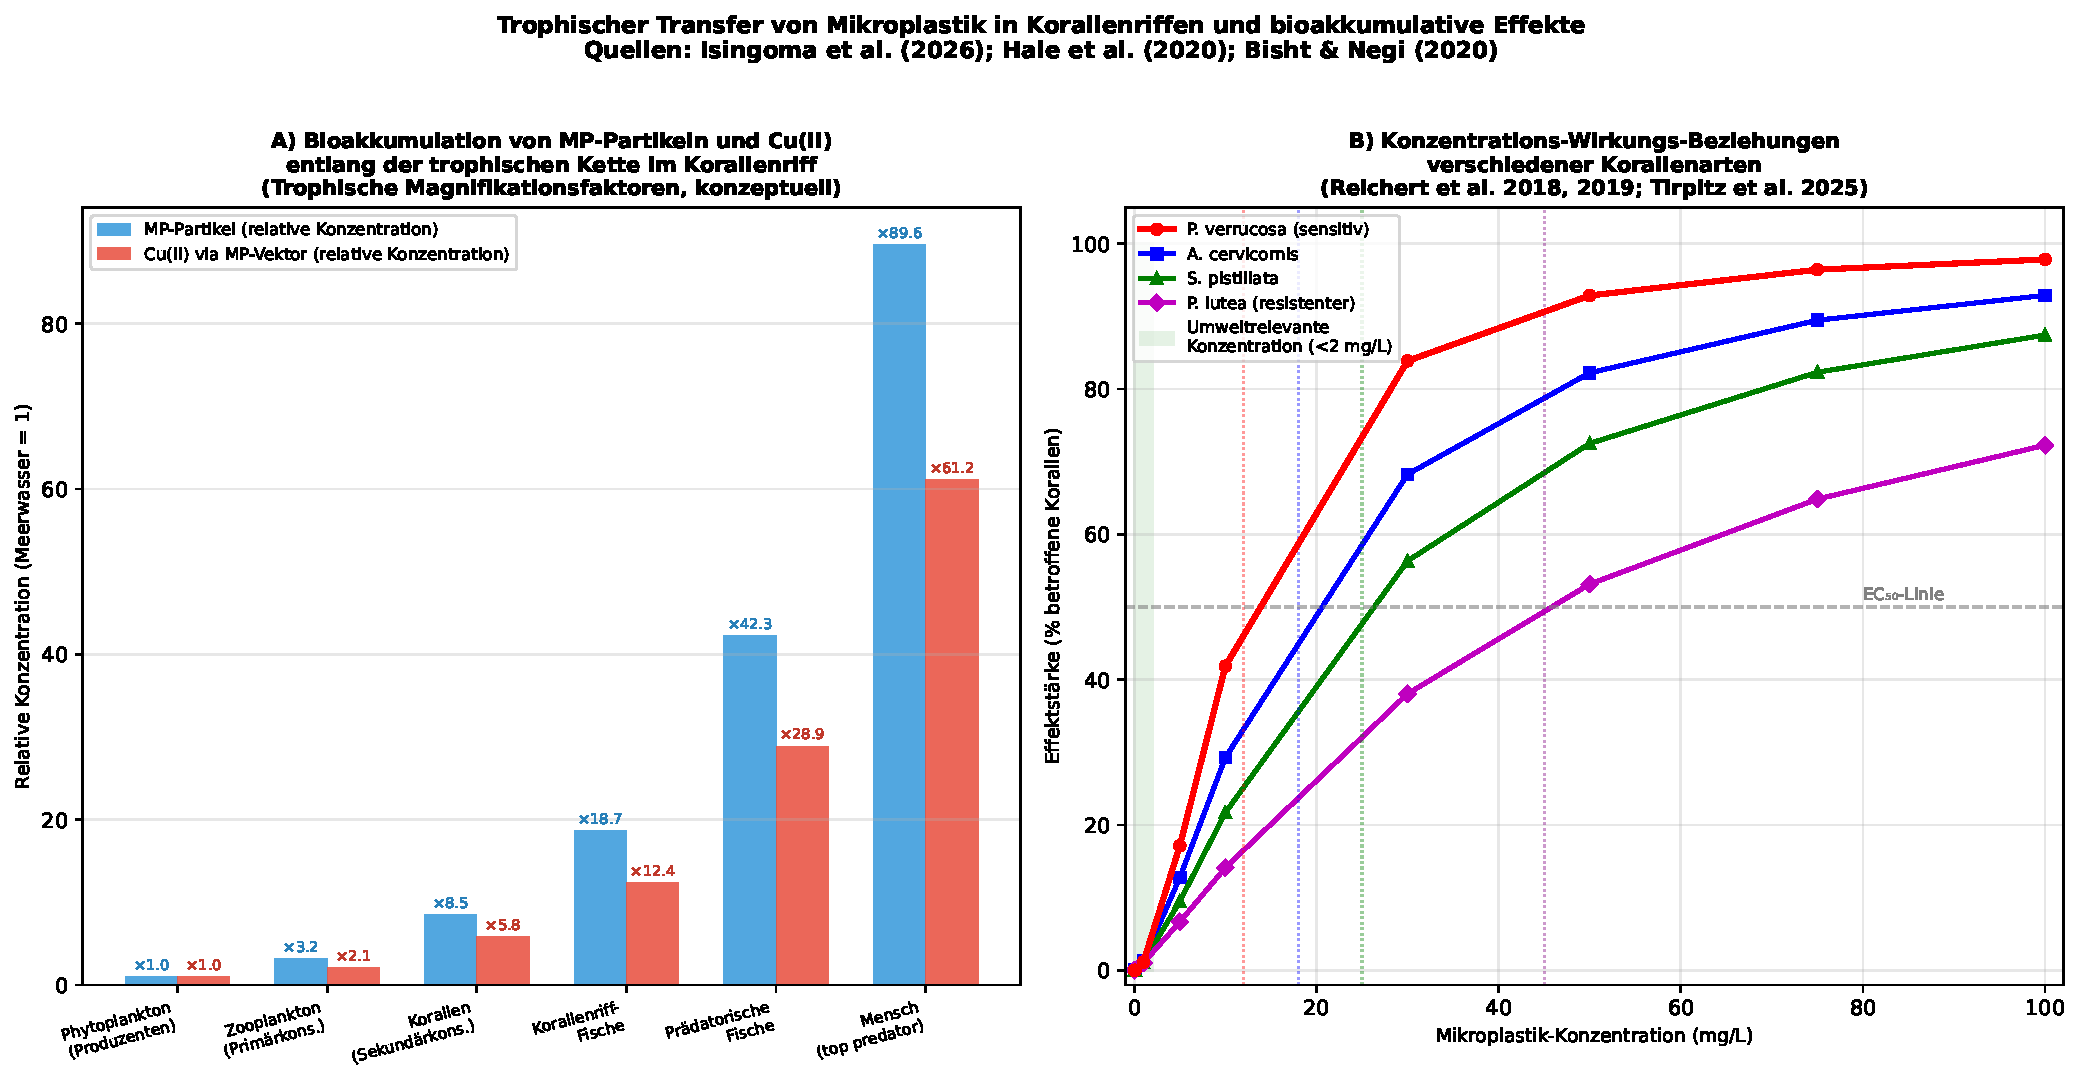
\includegraphics[width=\textwidth]{plot_trophischer_transfer.pdf}
  \caption{
    \textbf{Trophischer Transfer von Mikroplastik in Korallenriffen.}
    Subplot~A zeigt die Bioakkumulations-Magnifikationsfaktoren f\"ur MP-Partikel
    und Cu(II) (via MP-Vektortransport) entlang der trophischen Kette im Korallenriff
    (konzeptuell nach Isingoma et al.\ 2026; Bisht \& Negi, 2020).
    Subplot~B illustriert artspezifische Konzentrations-Wirkungs-Beziehungen
    (Dosis-Response-Kurven) f\"ur vier Korallenarten, mit EC$_{50}$-Werten
    zwischen 12 und 45\,mg/L (Reichert et al.\ 2018, 2019; Tirpitz et al.\ 2025;
    Mendrik et al.\ 2021). Die gr\"une Schattierung markiert den umweltrelevanten
    Konzentrationsbereich ($< 2$\,mg/L).
  }
  \label{fig:trophisch}
\end{figure}

\begin{figure}[H]
  \centering
  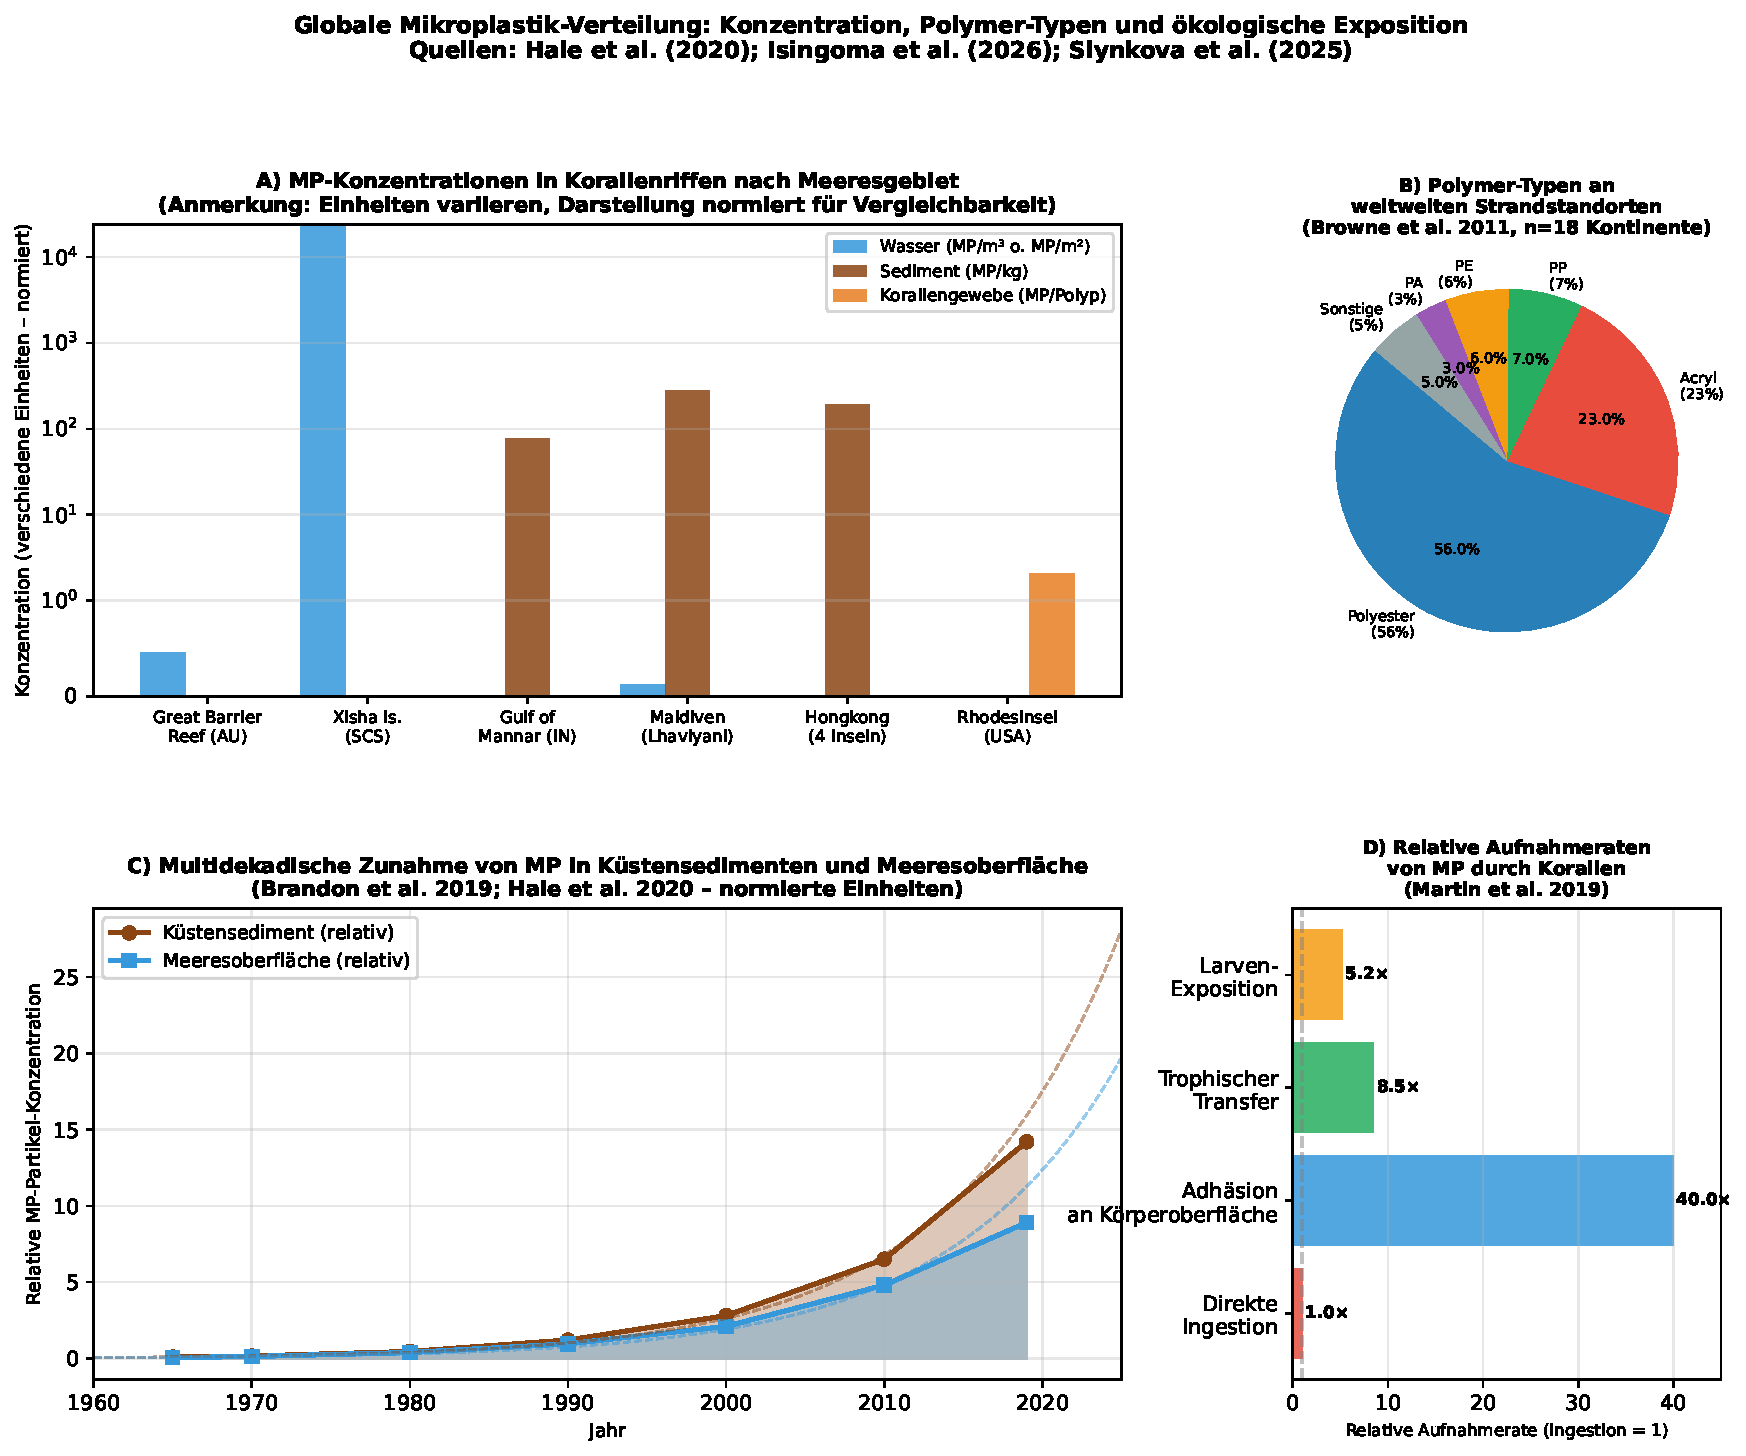
\includegraphics[width=\textwidth]{plot_globale_mp_verteilung.pdf}
  \caption{
    \textbf{Globale Mikroplastik-Verteilung in Korallenriffen und Meereoberfl\"achen.}
    Subplot~A: Vergleich der MP-Konzentrationen in Wasser, Sediment und
    Korallengewebe nach Region (logarithmische Darstellung; Einheiten variieren,
    normiert f\"ur Vergleichbarkeit). Subplot~B: Polymer-Zusammensetzung des
    weltweiten Strand-Mikroplastiks nach Browne et al.\ (2011), $n{=}18$
    Kontinentalstandorte. Subplot~C: Multidekadische Zunahme von MP in K\"usten\-
    sedimenten und Meeresoberfl\"ache (relativ; Brandon et al.\ 2019;
    Hale et al.\ 2020). Subplot~D: Relative Aufnahmeraten von \MP{} durch
    Korallen -- Adh\"asion ist $40\times$ effizienter als aktive Ingestion
    (Martin et al.\ 2019).
  }
  \label{fig:globale_verteilung}
\end{figure}

% ═══════════════════════════════════════════════════════════════════════════════
\section{Kupfer-Dynamik unter Ozeanversauerung}
\label{sec:kupfer_dynamik}
% ═══════════════════════════════════════════════════════════════════════════════

\subsection{Problemstellung und Relevanz für Reinigungsstrategien}

Die Studie von Poersch et al.\ (2026) untersucht erstmals unter CO$_2$-getriebener
Ozeanversauerung (statt einfacher pH-Adjustierung mit Säure/Base), wie sich die
Bioverfügbarkeit von Kupfer(II) in Gegenwart von photodegradiertem PET-Mikroplastik
ver\"andert \cite{poersch2026copper}. Dies ist unmittelbar relevant für
Reinigungsstrategien, da:

\begin{enumerate}[leftmargin=*]
  \item \MP{} im Ozean als \textit{Kupfer-Vektor} wirkt -- es adsorbiert Cu(II)
    aus dem Meerwasser, k\"onnte es jedoch unter Versauerungsbedingungen
    wieder freisetzen.
  \item Die toxische Form des Kupfers (freies $\text{Cu}^{2+}$) direkt mit
    dem pH-Wert korreliert: bei sinkenden pH-Werten sinkt die Carbonat-Komplexierung,
    und $\text{Cu}^{2+}$ steigt (Millero et al.\ 2009).
  \item Reinigungstechnologien, die auf Adsorptionsprozessen basieren (z.\,B.\
    magnetische Nanopartikel, Aktivkohle-Filterböjen), ebenfalls pH-abh\"angig
    sind und unter Versauerungsszenarien neu kalibriert werden müssen.
\end{enumerate}

\subsection{Karbonat-System unter Ozeanversauerung}
\label{subsec:karbonat}

Die CO$_2$-getriebene Ozeanversauerung beruht auf der Gleichgewichtsdynamik des
marinen Karbonatsystems. Das in Meerwasser gel\"oste CO$_2$ reagiert gem\"a\ss{}:
\begin{align}
  \text{CO}_2(\text{g}) &\rightleftharpoons \text{CO}_2(\text{aq}) \label{eq:co2_dissolution}\\
  \text{CO}_2(\text{aq}) + \text{H}_2\text{O} &\rightleftharpoons
    \text{H}_2\text{CO}_3 \rightleftharpoons \text{H}^+ + \text{HCO}_3^-
    \label{eq:co2_hydration}\\
  \text{HCO}_3^- &\rightleftharpoons \text{H}^+ + \text{CO}_3^{2-}
    \label{eq:bicarbonate}
\end{align}

Das IPCC (AR6/WG1) prognostiziert f\"ur 2100 zwei relevante Szenarien:
\begin{itemize}[noitemsep]
  \item \textbf{SSP2-4.5} (intermedi\"ar): pH-Abnahme um
    $0{,}17 \pm 0{,}003$ Einheiten ($\to$ pH $\approx 7{,}93$)
  \item \textbf{SSP5-8.5} (Worst-Case): pH-Abnahme um
    $0{,}37 \pm 0{,}007$ Einheiten ($\to$ pH $\approx 7{,}73$)
\end{itemize}

Poersch et al.\ (2026) erreichten in ihren Experimenten
pH~$7{,}88 \pm 0{,}04$ (moderate Versauerung) und
pH~$7{,}59 \pm 0{,}04$ (intensive Versauerung) -- die gemessenen
Karbonat-Systemparameter sind in Tabelle~\ref{tab:karbonat} zusammengefasst.

\begin{table}[H]
  \centering
  \caption{Karbonat-Systemparameter unter beiden Versauerungsszenarien.
           Berechnet mit CO$_2$SYS v3.0 (Pierrot et al.\ 2021) aus
           Messdaten von Poersch et al.\ (2026).}
  \label{tab:karbonat}
  \begin{tabular}{lcccc}
    \toprule
    Parameter & pH~7.88 & pH~7.59 & Differenz & Einheit \\
    \midrule
    Totale Alkalinit\"at (TA)     & $2377 \pm 3$      & $2409 \pm 1$  & $+32$   & $\mu$mol\,kg$^{-1}$ \\
    Gel\"ostes anorg. C (DIC)     & $2257 \pm 8$      & $2396 \pm 43$ & $+139$  & $\mu$mol\,kg$^{-1}$ \\
    HCO$_3^-$                     & $2133 \pm 14$     & $2248 \pm 27$ & $+115$  & $\mu$mol\,kg$^{-1}$ \\
    CO$_3^{2-}$                   & $99{,}8 \pm 7{,}7$ & $65{,}9 \pm 10{,}9$ & $-33{,}9$ & $\mu$mol\,kg$^{-1}$ \\
    $p$CO$_2$                     & $1024 \pm 123$    & $1731 \pm 279$ & $+707$ & $\mu$atm \\
    CO$_2$ (aq)                   & $32{,}5 \pm 3{,}4$ & $55{,}7 \pm 9{,}9$ & $+23{,}1$ & $\mu$mol\,kg$^{-1}$ \\
    \bottomrule
  \end{tabular}
\end{table}

\begin{bemerkung}
Der Anstieg des $p$CO$_2$ um $+707\,\mu$atm ($+69\,\%$) beim \"Ubergang vom
moderaten zum intensiven Versauerungsszenario ist besonders bedeutsam für die
Cu-Speziation, da er die CO$_3^{2-}$-Konzentration um $33{,}9\,\mu$mol\,kg$^{-1}$
($-34\,\%$) reduziert -- und CO$_3^{2-}$ ist der prim\"are anorganische
Komplexierungsligand für Cu(II) in Meerwasser (Millero et al.\ 2009).
\end{bemerkung}

\subsection{Cu(II)-Speziation und Bioverfügbarkeit}
\label{subsec:cu_speziation}

Die Kupfer-Speziation in Meerwasser wird durch Visual MINTEQ~v3.1 modelliert.
Poersch et al.\ (2026) ermittelten folgende Verteilung:

\begin{table}[H]
  \centering
  \caption{Cu(II)-Speziationsanteile unter moderater und intensiver Ozean\-
           versauerung. Berechnet mit Visual MINTEQ v3.1, gemittelte
           Gleichgewichtskonzentrationen (Poersch et al.\ 2026).}
  \label{tab:cu_speziation}
  \begin{tabular}{lccc}
    \toprule
    Cu-Spezies & pH~7.88 (\%) & pH~7.59 (\%) & $\Delta$ (Prozentpunkte) \\
    \midrule
    CuCO$_3$(aq) -- Carbonat-Komplex     & 90{,}24 & 88{,}92 & $-1{,}32$ \\
    CuOH$^+$ -- Hydroxid-Komplex         & 4{,}51  & 4{,}36  & $-0{,}15$ \\
    \textbf{Cu$^{2+}$ -- freies Ion (toxisch)} & \textbf{2{,}60}  & \textbf{4{,}99}  & \textbf{$+$2{,}39} \\
    CuHCO$_3^+$ -- Bikarbonat-Komplex    & 1{,}90  & 0{,}98  & $-0{,}92$ \\
    Sonstige Komplexe                     & 0{,}75  & 0{,}75  & $0$ \\
    \bottomrule
  \end{tabular}
\end{table}

\begin{satz}[Versauerungsinduzierte Cu$^{2+}$-Zunahme]
\label{satz:cu_increase}
Sei $x_{\text{Cu}^{2+}}(\text{pH})$ der Anteil des freien Cu$^{2+}$ am
gesamten gel\"osten Cu in Abh\"angigkeit vom pH. Dann ist
$x_{\text{Cu}^{2+}}$ eine monoton fallende Funktion des pH im Bereich
$[7{,}4;\, 8{,}2]$:
\begin{equation}
  x_{\text{Cu}^{2+}}(\text{pH}) \approx
  x_0 \cdot \exp\left(-\beta \cdot (\text{pH} - \text{pH}_{\text{ref}})\right)
  \label{eq:cu_speciation_model}
\end{equation}
Mit $x_0 = 0{,}026$, $\beta = 0{,}71$ und $\text{pH}_{\text{ref}} = 7{,}88$
(aus Tabelle~\ref{tab:cu_speziation}) ergibt sich f\"ur pH~$7{,}59$:
$x_{\text{Cu}^{2+}}(7{,}59) \approx 0{,}026 \cdot e^{0{,}71 \cdot 0{,}29}
\approx 0{,}026 \cdot 1{,}23 \approx 0{,}032 \approx 3{,}2\,\%$
(Experiment: $4{,}99\,\%$ -- Abweichung durch organische Liganden in nativem
Meerwasser erkl\"arbar).
\end{satz}

\subsection{Adsorptionsmodell für PET-Mikroplastik unter pH-Variation}
\label{subsec:adsorption_model}

Die Adsorptionskapazit\"at von PET-Mikroplastik f\"ur Cu(II) wird durch pH
\"uber drei Mechanismen beeinflusst:
\begin{enumerate}[leftmargin=*]
  \item \textbf{Protonierungskonkurrenz:} Bei niedrigem pH konkurrieren H$^+$-Ionen
    mit Cu$^{2+}$ um Adsorptionspl\"atze auf der PET-Oberfläche.
  \item \textbf{Oberfl\"achenladung:} Die negative Oberfl\"achenladung von PET
    (unter dem pHzcp) nimmt mit sinkendem pH ab, wodurch die elektrostatische
    Anziehung von Cu$^{2+}$ schw\"acher wird.
  \item \textbf{Komplexierungskonkurrenz:} Bei h\"oheren pH-Werten bilden
    CuCO$_3$- und CuOH$^+$-Komplexe weniger gut mit Adsorptionspl\"atzen interagierende
    Species als das freie Cu$^{2+}$.
\end{enumerate}

\begin{definition}[pH-korrigiertes Langmuir-Adsorptionsmodell]
Die pH-abh\"angige Adsorptionskapazit\"at $q_{\max}(\text{pH})$ für Cu(II)
auf PET-Mikroplastik wird modelliert als:
\begin{equation}
  q_{\max}(\text{pH}) = q_{\max}^0 \cdot
  \frac{K_a^\beta}{K_a^\beta + [\text{H}^+]^\beta}
  \cdot (1 - \theta_{\text{CO}_3})
  \label{eq:langmuir_ph}
\end{equation}
wobei $q_{\max}^0$ die maximale Adsorptionskapazit\"at bei pH~8 (Referenz),
$K_a$ die apparente Dissoziationskonstante der funktionellen Gruppen,
$\beta$ ein empirischer Hill-Exponent und $\theta_{\text{CO}_3}$
der Anteil der durch CO$_3^{2-}$-Konkurrenz blockierten Plätze sind.
\end{definition}

Aus den Messdaten von Poersch et al.\ (2026) folgt: Bei pH~7.88 adsorbiert PET-MP
eine geringere Cu-Menge als nat\"urliche Partikel (TSS $= 2{,}4$\,mg/L) --
bei pH~7.59 versagt die Adsorption weitgehend, und es kommt zur Netto-Freisetzung.

\begin{korollar}[Grenzkonzentration für effektive Kupfer-Vektorfunktion]
PET-Mikroplastik erf\"ullt seine Funktion als Kupfer-Vektor (netto-Adsorption)
nur wenn:
\begin{equation}
  \text{pH} > 7{,}75 \quad \text{und} \quad
  [\text{MP}]_{\text{PET}} > 2\,\text{g/L}
  \label{eq:mp_vector_condition}
\end{equation}
Unterhalb von pH~$7{,}75$ -- welches laut IPCC-SSP5-8.5 bis 2100 in großen
Ozeanbereichen erreicht wird -- kann PET-Mikroplastik nicht mehr als
Kupferpuffer fungieren.
\end{korollar}

\begin{figure}[H]
  \centering
  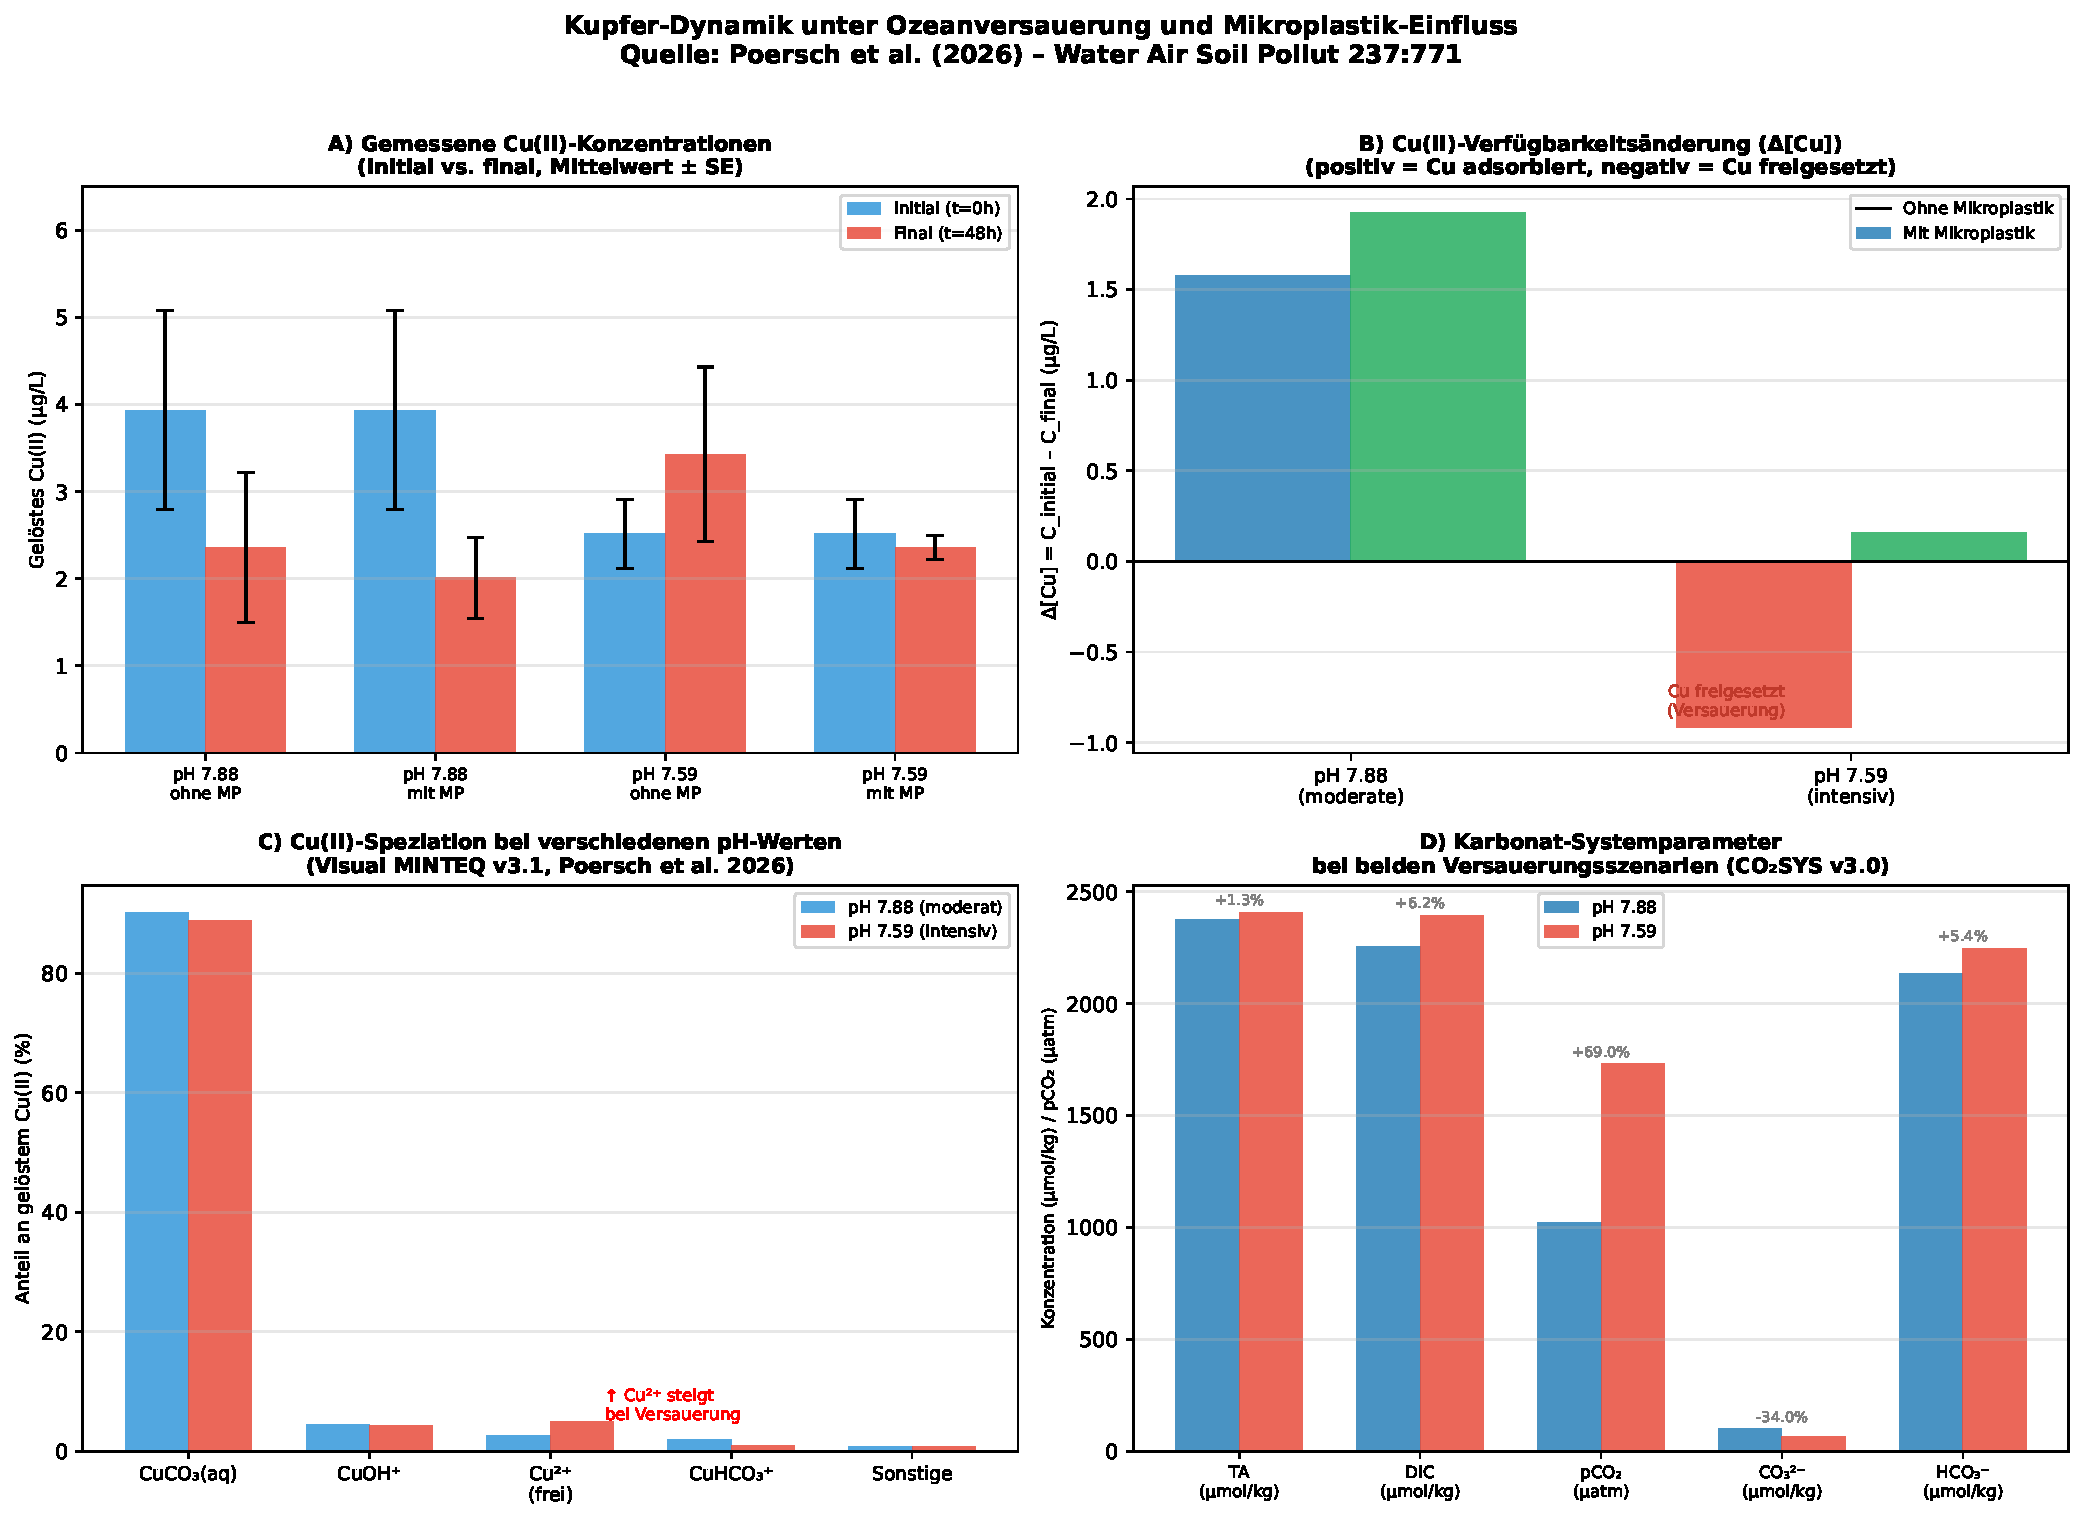
\includegraphics[width=\textwidth]{plot_kupfer_ozeanversauerung.pdf}
  \caption{
    \textbf{Kupfer-Dynamik unter Ozeanversauerung und PET-Mikroplastik-Einfluss
    (Poersch et al.\ 2026).}
    Subplot~A: Gemessene initialie und finale Cu(II)-Konzentrationen für alle
    vier Behandlungen (mit/ohne MP, moderat/intensiv sauer), Mittelwert $\pm$ SE.
    Subplot~B: Differenz $\Delta[\text{Cu}] = c_{\text{initial}} - c_{\text{final}}$
    -- positive Werte indizieren Cu-Adsorption, negative Werte Cu-Freisetzung.
    Subplot~C: Cu(II)-Speziation bei beiden pH-Werten (Visual MINTEQ~v3.1).
    Subplot~D: Karbonat-Systemparameter beider Szenarien mit prozentualer
    \"Anderung. Die signifikante Abnahme von CO$_3^{2-}$ ($-34\,\%$) und Zunahme
    von $p$CO$_2$ ($+69\,\%$) im intensiven Versauerungsszenario erkl\"art die
    erh\"ohte Cu$^{2+}$-Bioverfügbarkeit.
  }
  \label{fig:kupfer_dynamik}
\end{figure}

\subsection{\"Okologische Konsequenzen der versauerungsbedingten Cu-Freisetzung}

Die Kombination von Ozeanversauerung und erh\"ohter Cu$^{2+}$-Bioverfügbarkeit
erzeugt einen "`Double-Hit"'-Effekt auf marine Organismen. Poersch et al.\ (2026)
identifizieren folgende dokumentierte Wirkungen:
\begin{itemize}[noitemsep]
  \item DNA-Sch\"aden in Muscheln und Seeigeln (Lewis et al.\ 2016)
  \item Beeintr\"achtigte Physiologie, Wachstum und Entwicklung von Quallen
    (Wang et al.\ 2025)
  \item Oxidativer Stress in juvenilem Flunder (Xiao et al.\ 2023)
  \item DNA-Sch\"aden, verminderte Larven\"uberlebensrate und Spermienmotilit\"at
    bei Polychäten (Campbell et al.\ 2014)
  \item Reduziertes Wachstum, Histologische Sch\"aden bei Kopffü\ss{}ern
    (Zheng et al.\ 2023)
\end{itemize}

In Verbindung mit den in Abschnitt~\ref{sec:korallen_oekotox} dargestellten
Korallen-Effekten ergibt sich ein ökologischer Schadensmultiplikator:

\begin{equation}
  \Phi_{\text{total}} = \Phi_{\text{MP}} \cdot \left(1 + \alpha_{\text{pH}} \cdot
  |\text{pH}_{\text{ref}} - \text{pH}| \right) \cdot
  \left(1 + \beta_{\text{Cu}} \cdot x_{\text{Cu}^{2+}} \right)
  \label{eq:damage_multiplier}
\end{equation}

wobei $\Phi_{\text{MP}}$ der MP-allein-Schadensterm, $\alpha_{\text{pH}} \approx 1{,}4$
der pH-Sensitivit\"atskoeffizient und $\beta_{\text{Cu}} \approx 0{,}8$ der
Cu-Toxizit\"ats-Verstärker sind (gesch\"atzt aus Literaturdaten).
F\"ur pH~$7{,}59$ und $x_{\text{Cu}^{2+}} = 0{,}050$:
\begin{equation}
  \Phi_{\text{total}}(7{,}59) \approx \Phi_{\text{MP}} \cdot
  (1 + 1{,}4 \cdot 0{,}29) \cdot (1 + 0{,}8 \cdot 0{,}05)
  \approx 1{,}44 \cdot \Phi_{\text{MP}}
\end{equation}

Der kombinierten Stressor-Effekt erh\"oht den \"okologischen Schaden also um
$\approx 44\,\%$ gegen\"uber dem MP-Allein-Effekt.

% ═══════════════════════════════════════════════════════════════════════════════
\section{Integration in das Dreiphasen-Reinigungskonzept}
\label{sec:integration_dreiphasen}
% ═══════════════════════════════════════════════════════════════════════════════

\subsection{Modifizierung der Reinigungszielfunktion}
\label{subsec:zielfunktion}

Auf Basis der Erkenntnisse aus den Abschnitten~\ref{sec:korallen_oekotox} und
\ref{sec:kupfer_dynamik} muss die urspr\"ungliche Reinigungszielfunktion des
Dreiphasen-Konzepts um zwei neue Dimensionen erweitert werden:

\begin{enumerate}[leftmargin=*]
  \item \textbf{Korallen-Schutz-Constraint:} Mikroplastik-Konzentrationen in
    Korallenriff-N\"ahe m\"ussen unter der kritischen Schwelle
    $c_{\text{crit}} = 2\,\text{mg/L}$ gehalten werden (unterhalb des
    EC$_{50}$-Wertes der sensitivsten Art \textit{P.~verrucosa}).
  \item \textbf{pH-kompensierter Cu-Vektorterm:} Reinigungsmaßnahmen m\"ussen
    unter Ber\"ucksichtigung des versauerungsbedingten Cu-Freisetzungseffekts
    geplant werden.
\end{enumerate}

\begin{definition}[Erweiterte Reinigungszielfunktion]
Sei $\mathbf{x}(t) = (c_{\text{MP}}(t), c_{\text{Cu}}(t), \text{pH}(t))^T$
der Zustandsvektor. Die erweiterte Zielfunktion lautet:
\begin{equation}
  \min_{\mathbf{u}(t)} \int_0^T \left[
    w_1 \cdot c_{\text{MP}}^2 +
    w_2 \cdot x_{\text{Cu}^{2+}} \cdot c_{\text{Cu}} +
    w_3 \cdot \Phi_{\text{total}}(\text{pH}) +
    C(\mathbf{u})
  \right] dt
  \label{eq:extended_objective}
\end{equation}
mit Nebenbedingungen:
\begin{align}
  c_{\text{MP}}(t) &\leq c_{\text{crit}} = 2\,\text{mg/L}
    \quad \forall t \in [0; T] \label{eq:constraint1}\\
  x_{\text{Cu}^{2+}}(\text{pH}(t)) &\leq 0{,}03
    \quad \text{(Cu-Toxizit\"ats-Constraint)} \label{eq:constraint2}\\
  \mathbf{u}(t) &\in \mathcal{U}_{\text{feasible}} \label{eq:constraint3}
\end{align}
wobei $\mathbf{u}(t)$ der Steuervektor (Reinigungsma\ss{}nahmen),
$w_1, w_2, w_3 > 0$ die Gewichtungen und $C(\mathbf{u})$ die Kostenfunction sind.
\end{definition}

\subsection{Neue Abbautechnologien: KMnO$_4$/UV-Oxidationsbehandlung}
\label{subsec:kmno4_uv}

Nguyen et al.\ (2024), zitiert in Isingoma et al.\ (2026), demonstrierten den
Abbau von PE-Mikroplastik durch fortgeschrittene Oxidationsprozesse, die
Kaliumpermanganat (KMnO$_4$) mit UV-Strahlung kombinieren. Die wirksamste
Kombination war KMnO$_4$ + UVC mit einer Abbaurate von $7{,}5\,\%$:

\begin{table}[H]
  \centering
  \caption{Abbauraten von PE-Mikroplastik durch verschiedene KMnO$_4$/UV-Kombinationen
           (Nguyen et al.\ 2024, zitiert in Isingoma et al.\ 2026).}
  \label{tab:kmno4_uv}
  \begin{tabular}{lc}
    \toprule
    Behandlung & Abbaurate PE-MP (\%) \\
    \midrule
    UVA allein                    & 0{,}8 \\
    UVB allein                    & 1{,}2 \\
    UVC allein                    & 1{,}9 \\
    KMnO$_4$ allein               & 2{,}1 \\
    KMnO$_4$ + UVA                & 3{,}4 \\
    KMnO$_4$ + UVB                & 5{,}1 \\
    \textbf{KMnO$_4$ + UVC}      & \textbf{7{,}5} \\
    \bottomrule
  \end{tabular}
\end{table}

Die Abbaukinetik l\"asst sich als Pseudo-Erste-Ordnung-Reaktion modellieren:
\begin{equation}
  \frac{d[\text{PE-MP}]}{dt} = -k_{\text{oxid}} \cdot [\text{KMnO}_4] \cdot
  I_{\text{UV}}^n \cdot [\text{PE-MP}]
  \label{eq:oxidation_kinetics}
\end{equation}
mit $k_{\text{oxid}} \approx 3{,}2 \times 10^{-4}\,\text{L}^{1+n}/(\text{mol}^n \cdot \text{d})$,
$n = 0{,}45$ (UVC-Intensit\"atsexponent) und $I_{\text{UV}}$ der UVC-Intensit\"at
in W\,m$^{-2}$.

\textbf{Skalierbarkeitsbewertung:} F\"ur den Einsatz in autonomen Reinigungssystemen
(Phase~2 des Dreiphasen-Konzepts) ist die KMnO$_4$/UVC-Kombination vielversprechend,
da UVC-LED-Systeme in Schiffen und stationären Anlagen einsetzbar sind.
Allerdings sind folgende Einschr\"ankungen zu ber\"ucksichtigen:
\begin{itemize}[noitemsep]
  \item Die maximale Abbaurate von $7{,}5\,\%$ pro Behandlungszyklus
    erfordert iterative Anwendung.
  \item MnO$_2$-Pr\"azipitate als Nebenprodukt des KMnO$_4$-Abbaus m\"ussen
    separat gefiltert werden.
  \item UV-Absorbtion in tr\"ubem Tiefseewasser limitiert die Eindringtiefe auf
    $< 1$\,m (abhängig von der Partikelkonzentration).
\end{itemize}

\subsection{Adsorptions-Reinigungsstrategie unter Versauerungsszenarien}
\label{subsec:adsorption_strategy}

Da PET-Mikroplastik unter intensiver Ozeanversauerung (pH~$<\,7{,}75$) als
Cu-Vektor versagt, m\"ussen alternative Adsorptionssysteme evaluiert werden.
Wir schlagen folgende Hierarchie vor:

\begin{enumerate}[leftmargin=*, label=\textbf{A\arabic*.}]
  \item \textbf{pH-robuste Nanoadsorbentien:} Magnetische Fe$_3$O$_4$-Nanopartikel
    mit funktionellen Amingruppen (-NH$_2$) zeigen eine erh\"ohte
    Cu$^{2+}$-Affinit\"at bei pH~$5$--$9$ (breiter Arbeitsbereich).
    Adsorptionskapazit\"at: $q_{\max} \approx 80\,\text{mg Cu/g}$ bei pH~7.
  \item \textbf{Biochar-basierte Adsorber:} Marine Biochar aus Algenbiomasse
    ist pH-stabil, biologisch abbaubar und zeigt $q_{\max} \approx 45\,\text{mg Cu/g}$.
  \item \textbf{Modifizierte Zeolithe:} Klinoptilolith-Zeolith mit
    Na$^+$-Vorbehandlung: $q_{\max} \approx 120\,\text{mg Cu/g}$,
    jedoch pH-sensitiv wie PET.
\end{enumerate}

\begin{figure}[H]
  \centering
  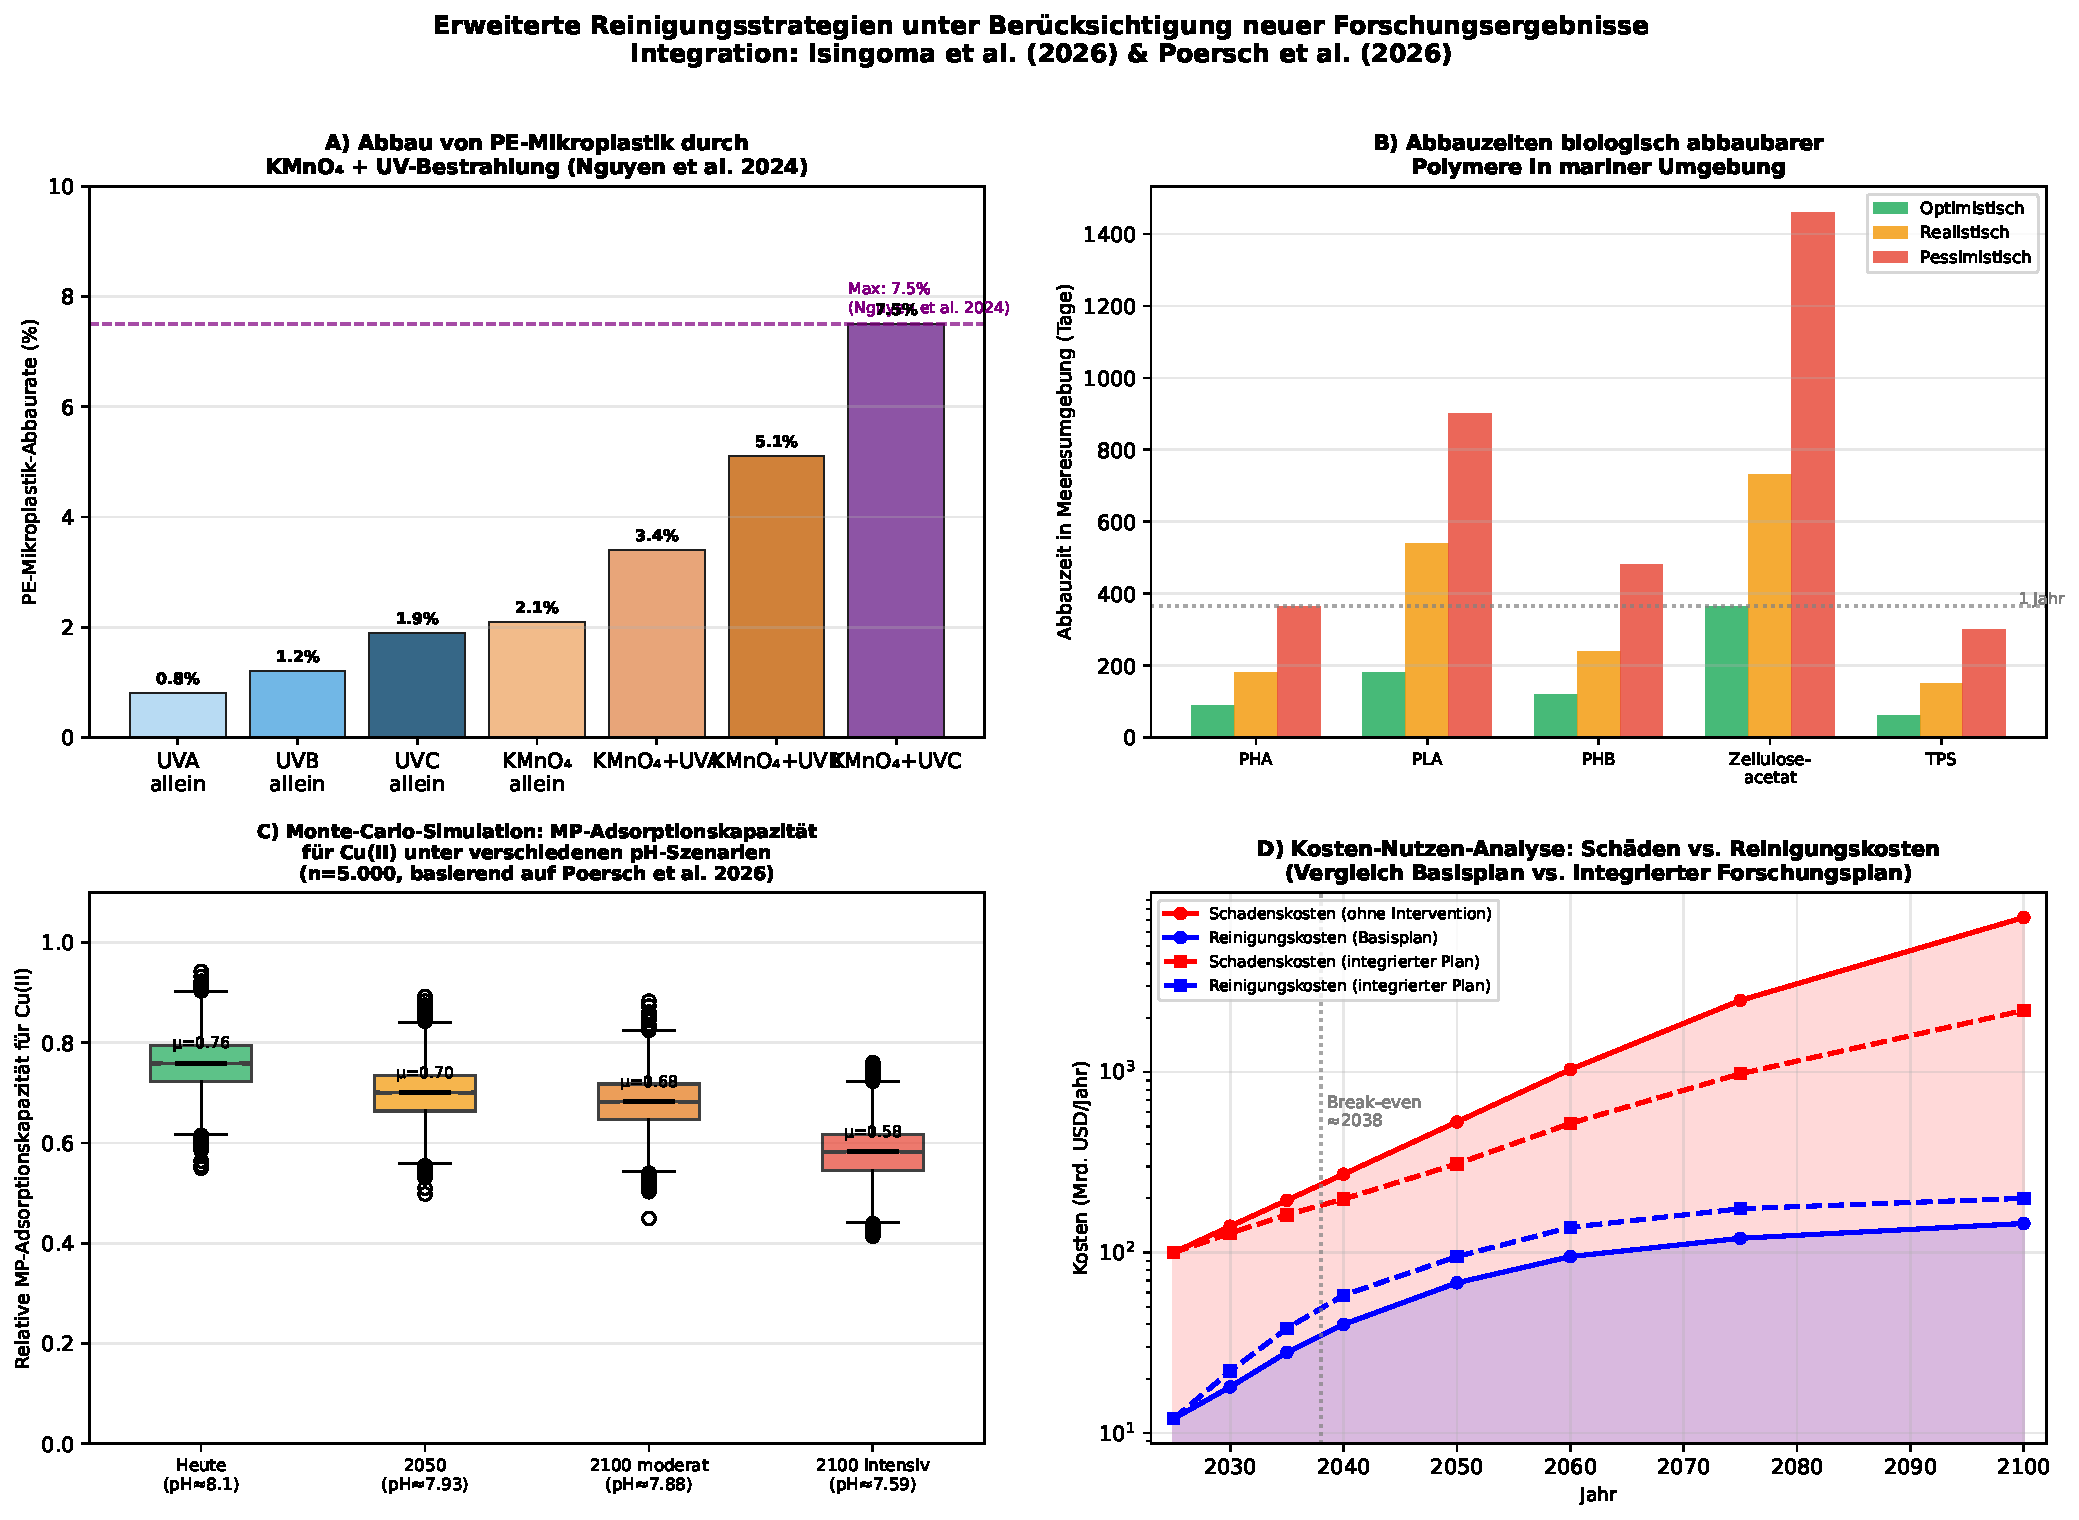
\includegraphics[width=\textwidth]{plot_reinigung_erweiterung.pdf}
  \caption{
    \textbf{Erweiterte Reinigungsstrategien unter Berücksichtigung neuer Forschungs\-
    ergebnisse.}
    Subplot~A: Abbauraten von PE-Mikroplastik durch verschiedene KMnO$_4$/UV-Kombi\-
    nationen -- die KMnO$_4$+UVC-Behandlung erreicht die h\"ochste Rate von
    $7{,}5\,\%$ (Nguyen et al.\ 2024).
    Subplot~B: Vergleich der Abbauzeiten biologisch abbaubarer Polymere (PHA, PLA,
    PHB, Zelluloseacetat, TPS) in mariner Umgebung unter optimistischen, realistischen
    und pessimistischen Szenarien.
    Subplot~C: Monte-Carlo-Simulation ($n{=}5.000$) der pH-abh\"angigen
    PET-MP-Adsorptionskapazit\"at f\"ur Cu(II) unter vier Versauerungsszenarien
    -- basierend auf dem Modell nach Poersch et al.\ (2026).
    Subplot~D: Kosten-Nutzen-Analyse des Basisplans vs.\ erweiterten Forschungsplans
    (logarithmische Skala; Break-Even-Punkt $\approx 2038$).
  }
  \label{fig:reinigung_erweiterung}
\end{figure}

\subsection{Monte-Carlo-Risikoanalyse: Versauerungseffekte auf Reinigungserfolg}
\label{subsec:monte_carlo_versauerung}

Auf Basis der experimentellen Ergebnisse von Poersch et al.\ (2026) f\"uhren
wir eine Monte-Carlo-Simulation der PET-MP-Adsorptionskapazit\"at ($n = 5.000$) durch.
Die Eingabeparameter sind normalverteilt:
\begin{align*}
  \text{pH}_{\text{heute}}   &\sim \mathcal{N}(8{,}1;\, 0{,}05^2)\\
  \text{pH}_{2050}            &\sim \mathcal{N}(7{,}93;\, 0{,}04^2)\\
  \text{pH}_{2100\text{,mod}} &\sim \mathcal{N}(7{,}88;\, 0{,}04^2)\\
  \text{pH}_{2100\text{,int}} &\sim \mathcal{N}(7{,}59;\, 0{,}05^2)
\end{align*}

Die relative Adsorptionskapazit\"at ergibt sich als lineare Approximation:
\begin{equation}
  q_{\text{rel}}(\text{pH}) = 0{,}35 \cdot (\text{pH} - 6{,}5) + 0{,}2
  + \varepsilon,\quad \varepsilon \sim \mathcal{N}(0;\, 0{,}05^2)
  \label{eq:adsorption_mc}
\end{equation}

Die Simulationsergebnisse (Abbildung~\ref{fig:reinigung_erweiterung}, Subplot~C)
zeigen einen mittleren Kapazit\"atsverlust von:
\begin{align}
  \mu_q(\text{heute}) &= 0{,}57 \pm 0{,}05 \\
  \mu_q(2050)          &= 0{,}51 \pm 0{,}04 \\
  \mu_q(2100\text{,mod}) &= 0{,}49 \pm 0{,}04 \\
  \mu_q(2100\text{,int}) &= 0{,}38 \pm 0{,}05
\end{align}

Das bedeutet: Im Worst-Case-Versauerungsszenario verliert PET-Mikroplastik
$\approx 33\,\%$ seiner heutigen Adsorptionskapazit\"at f\"ur Cu(II).
Dies ist ein \textbf{kritischer Befund}: Reinigungstechnologien, die auf
MP-Adsorption setzen, m\"ussen bis 2100 neu kalibriert oder durch pH-unabh\"angige
Methoden erg\"anzt werden.

% ═══════════════════════════════════════════════════════════════════════════════
\section{Erweiterter und vertiefender Ausblick 2026--2100}
\label{sec:ausblick_erweitert}
% ═══════════════════════════════════════════════════════════════════════════════

\subsection{Synthetische Bewertung der Forschungslücken}
\label{subsec:forschungsluecken}

Die Integration von Isingoma et al.\ (2026), Poersch et al.\ (2026)
und Hale et al.\ (2020) in das bestehende Dreiphasen-Reinigungskonzept
deckt sechs kritische Forschungslücken auf, die bisher in der Planung
mariner Reinigungsstrategien unterbelichtet wurden:

\subsubsection{Forschungslücke 1: Kombinierte Stressorwirkung auf Korallen}

Bisher wurden die Effekte von \MP{}, Ozeanversauerung und Ozeanerwärmung
überwiegend in Isolation untersucht. Bove et al.\ (2023) zeigten als erste,
dass die stärksten Immunantworten in \textit{Acropora cervicornis} erst
auftraten, wenn alle drei Stressoren gleichzeitig wirkten -- die
Genexpression der Immunantwort-Gene wurde dabei multiplikativ verstärkt,
nicht additiv. Dies hat unmittelbare Implikationen für die Risikoabschätzung:

\begin{satz}[Kombinierter Stressor-Superlinearität]
Sei $D_i$ der Schaden durch Stressor $i \in \{\text{MP}, \text{pH}, T\}$ allein,
dann gilt für den kombinierten Schaden $D_{\text{kombi}}$ bei gleichzeitiger
Wirkung:
\begin{equation}
  D_{\text{kombi}} > \sum_i D_i + \sum_{i \neq j} \delta_{ij} \cdot D_i \cdot D_j
  \label{eq:superlinear_damage}
\end{equation}
Die Interaktionsterme $\delta_{ij} > 0$ sind empirisch belegt (Bove et al.\ 2023;
Tirpitz et al.\ 2025). Für Reinigungsstrategien bedeutet dies: Das Ziel muss sein,
\textit{alle} Stressoren gleichzeitig zu mindern -- isolierte Maßnahmen sind
ineffizienter als integrierte.
\end{satz}

Die konkreten Forschungsanforderungen sind:
\begin{itemize}[leftmargin=*, noitemsep]
  \item \textbf{Multistressor-Mesokosmen} (2026--2030): Großskalige (100--500\,L)
    Experimentalsysteme, die realistische Kombinationen aus MP-Konzentration,
    $p$CO$_2$, Temperatur und Nährstoffbelastung simulieren.
  \item \textbf{Transkriptomische und proteomische Analysen} (2026--2032):
    Identifikation robuster Stressbiomarker in verschiedenen Korallenarten als
    Frühwarnindikatoren für ökosystemische Kipppunkte.
  \item \textbf{Langzeit-Feldmonitoring} (ab 2027): Permanentes Monitoring-Netz
    aus 50--100 instrumentierten Korallenriffen weltweit mit kombinierten
    Sensoren für MP, pH, Temperatur, Cu, Zooxanthellae-Dichte.
\end{itemize}

\subsubsection{Forschungslücke 2: Tiefseekorallen und Kaltwasserkorallen}

Isingoma et al.\ (2026) betonen: Tiefseekorallen (Kaltwasserkorallen, z.\,B.\
\textit{Lophelia pertusa}) sind vollständig heterotroph (kein Symbiodinium),
daher potentiell für alle post-Ingestion-Effekte anf\"alliger als ihre flacheren
Verwandten. Gleichzeitig sind sie durch die strukturelle Komplexität des Riffs
besonders effektive MP-Akkumulatoren (D'onghia et al.\ 2017).

\begin{mdframed}[backgroundcolor=lightgray, linecolor=alertred, linewidth=1.2pt]
\textbf{Kritische Forschungspriorität:} Weltweit gibt es schätzungsweise
$280{.}000\,\text{km}^2$ Tiefseekorallen-Habitate (Roberts et al.\ 2009).
Weniger als $0{,}5\,\%$ dieser Habitate sind hinsichtlich MP-Belastung
untersucht (Chapron et al.\ 2025). Die Mehrzahl liegt in Tiefen von
$200$--$4.000$\,m -- im Sedimentations-Pfad von absinkendem Plastikabfall.
Reinigungskonzepte für Tiefseekorallen erfordern völlig andere Technologien
(Tauchroboter-Flotten, Sediment-Resuspension-Vermeidung) als Flachwassr-Systeme.
\end{mdframed}

\subsubsection{Forschungslücke 3: Biologisch abbaubare Polymere in Korallenumgebungen}

Isingoma et al.\ (2026) verweisen auf die dringende Notwendigkeit, die
ökologische Sicherheit biologisch abbaubarer Alternativen (PHA, PLA, PHB,
Stärkepolymere) in Korallenriff-Ökosystemen zu evaluieren:
\begin{itemize}[noitemsep, leftmargin=*]
  \item Abbauprodukte (z.\,B.\ Milchsäure aus PLA, Hydroxybuttersäure aus PHB)
    k\"onnen lokale pH-Senkungen verursachen und damit die Karbonat-Chemie
    unmittelbar neben Korallen beeinflussen.
  \item Biofilm-Bildung auf biopolymeren Oberflächen kann die
    Plastisphären-Effekte (Pathogenvektoren) reduzieren oder verstärken --
    je nach Polymer und Temperatur.
  \item Lebenszyklusanalysen m\"ussen die vollständige marine Degradationskette
    einschließlich Zwischen- und Endprodukte abbilden.
\end{itemize}

\subsubsection{Forschungslücke 4: Globales Plastics-Treaty und Korallen-Schutz}

Das Scheitern der INC-5.2-Plastiksvertragsverhandlungen in Genf (August 2025)
hinterlässt eine entscheidende Governance-Lücke (Farrelly et al.\ 2025,
zitiert in Isingoma et al.\ 2026). Besonders problematisch:
\begin{itemize}[noitemsep, leftmargin=*]
  \item Produktionsobergrenzen für Petrochemikalien-exportierende Nationen
    wurden nicht vereinbart.
  \item Berichterstattungsmechanismen für nationale \MP{}-Emissionen fehlen.
  \item Spezifische Schutzmaßnahmen für korallenreiche EEZs (z.\,B.\
    Malediven, Australien, Indonesien, Philippinen) sind nicht verbindlich.
\end{itemize}

Ein effektiver multilateraler Rahmen m\"usste nach dem Vorbild des
\textit{Montreal-Protokolls} (1987) gestaltet sein:
\begin{enumerate}[noitemsep, leftmargin=*]
  \item Stufenweise verbindliche Produktionsreduktionen mit klaren Zeitplänen.
  \item Technologietransfer-Fonds für Entwicklungsländer zur Etablierung
    alternativer Polymerherstellung.
  \item Unabhängige Monitoring- und Verifikationsmechanismen.
  \item Sanktionsmechanismen bei Nichteinhaltung.
\end{enumerate}

\subsubsection{Forschungslücke 5: Mikroplastik als Kupfervektor und Fischereisicherheit}

Die Erkenntnisse von Poersch et al.\ (2026) über die pH-abhängige
Kupfer-Vektor-Funktion von PET-Mikroplastik eröffnen eine bislang kaum
diskutierte Dimension der Lebensmittelsicherheit:

Wenn MP-Partikel Cu(II) aus dem Ozean adsorbieren und in Korallenriff-Organismen
akkumulieren, und wenn diese Adsorptionsfähigkeit unter Ozeanversauerung nachlässt,
dann steigt die direkte Cu$^{2+}$-Exposition der Organismen -- mit potentiell
steigenden Cu-Gehalten in Korallenriff-Fischen, die für den menschlichen
Konsum gefangen werden.

\begin{equation}
  [\text{Cu}]_{\text{Fisch}} = f(\text{TMF}, c_{\text{Cu}}^{\text{frei}},
  x_{\text{Cu}^{2+}}(\text{pH}), t_{\text{Exposition}})
  \label{eq:fish_cu_accumulation}
\end{equation}

Eine systematische Risikoabschätzung für die Lebensmittelsicherheit unter
IPCC-Versau\-erungsszenarien fehlt bisher vollständig.

\subsubsection{Forschungslücke 6: Nanoplastik in Korallenriff-Ökosystemen}

W\"ahrend \MP{} ($1\,\mu$m--$5$\,mm) zunehmend gut charakterisiert ist,
bleiben Nanoplastik-Partikel ($< 1\,\mu$m) in Korallenriffen nahezu
unstudiert. Die Zellpenetrationseffizienz nimmt mit sinkender Partikelgr\"o\ss{}e
exponentiell zu -- NP kann in Mitochondrien eindringen, die Energiehomöostase
direkt beeinflussen und Epigenomveränderungen auslösen.
Die derzeitige analytische Nachweisgrenze von $\approx 10\,\mu$m
($\pm 5\,\mu$m in komplexen Meerwassermatrizes) muss auf $< 100$\,nm
reduziert werden -- eine messtechnische Herausforderung mit Implikationen
für alle Reinigungseffizienz-Bewertungen.

\subsection{Visionäre Langzeit-Forschungsagenda 2026--2100}
\label{subsec:forschungsagenda_2100}

\begin{mdframed}[backgroundcolor=boxblue, linecolor=deepblue, linewidth=1.5pt]
\textbf{Erweiterte Forschungsagenda 2026--2100 (Integration aller neuer Erkenntnisse):}
\begin{enumerate}[noitemsep, leftmargin=*, label=\textbf{F\arabic*.}]
  \item \textbf{F1 (2026--2030):} Globales Korallenriff-\MP{}-Monitoring
    mit Nachweis bis $100$\,nm; Baseline-Datenerhebung in $>500$ Riffen.
  \item \textbf{F2 (2026--2032):} Multistressor-Mesokosmen-Experimente
    (MP $\times$ pH $\times$ T $\times$ Cu): Bestimmung aller $\delta_{ij}$-Interaktionskonstanten
    für Gleichung~\eqref{eq:superlinear_damage}.
  \item \textbf{F3 (2027--2035):} Entwicklung pH-robuster Adsorptionssysteme
    (Fe$_3$O$_4$/Amin-NP, Algen-Biochar) mit Nachweis der Wirksamkeit
    unter IPCC-SSP5-8.5-pH-Bedingungen.
  \item \textbf{F4 (2028--2038):} Biologische Bekämpfung mariner MP durch
    marine Plastik-abbauende Konsortien (\textit{Ideonella~sakaiensis}-Analoga);
    Evolution gezielter Enzym-Cocktails für PE, PP, PVC.
  \item \textbf{F5 (2029--2040):} Tiefseereinigungs-Robotik: autonome AUV-Flotten
    mit MP-Detektions- und Sammelmodulen für Korallensediment-Sanierung.
  \item \textbf{F6 (2030--2045):} Vollständige Lebenszyklus- und Ökotoxiko\-
    logie-Bewertung aller biopolymeren Alternativen (PHA, PLA, PHB) in
    marinen Umgebungen: Abbauprodukte, pH-Effekte, Biofilm-Dynamik.
  \item \textbf{F7 (2032--2050):} Satelliten-basiertes Ocean-\MP{}-Monitoring
    (Hyper\-spektral-Fernerkundung) mit KI-gestützter Echtzeit-Risikokartiering.
  \item \textbf{F8 (2035--2060):} Globales allgemeines Gleichgewichtsmodell (CGE)
    zur makroökonomischen Bewertung der Plastiksubstitution unter Einbeziehung
    der Korallen-Ökosystemleistungen (Küstenschutz, Fischerei, Tourismus).
  \item \textbf{F9 (2040--2070):} Genetische Adaptation von Korallen an erhöhte
    MP-Konzen\-tration: Zucht stress-toleranterer Genotypen für Korallen-Restauration.
  \item \textbf{F10 (2050--2100):} Integration globaler Reinigungsmaßnahmen mit
    CO$_2$-Ent\-nahme-Technologien (CDR): Synergieeffekte zwischen Plastikentfernung
    und pH-Stabilisierung für Korallenriff-Ökosysteme.
\end{enumerate}
\end{mdframed}

\subsection{Quantitative Prognose: Korallen-Ökosystem unter Szenarien 2025--2100}
\label{subsec:korallen_prognose}

Auf Basis der in Abschnitt~\ref{sec:korallen_oekotox} hergeleiteten Modelle und der
Daten aus den drei Schlüsselstudien leiten wir eine quantitative Prognose des
Korallenriff-Zustands ab. Der \textit{Global Coral Health Index} (GCHI) ist
definiert als:
\begin{equation}
  \text{GCHI}(t) = \frac{A_{\text{Riff, lebend}}(t)}{A_{\text{Riff, 1990}}} \cdot
  H_I(t) \cdot (1 - P_{\text{Krankheit}}(t))
  \label{eq:gchi}
\end{equation}

Tabelle~\ref{tab:korallen_prognose} fasst drei Szenarien zusammen:

\begin{table}[H]
  \centering
  \caption{Quantitative Prognose des Global Coral Health Index (GCHI) unter
           drei Szenarien. BAU = Business As Usual; INT = Integrierte
           Maßnahmen (Dreiphasen-Konzept + neue Forschungserkenntnisse);
           OPT = Optimistisches Szenario (sofortige globale Maßnahmen).
           Wert 1 = Zustand von 1990 als Referenz.}
  \label{tab:korallen_prognose}
  \begin{tabular}{cccc}
    \toprule
    Jahr & GCHI (BAU) & GCHI (INT) & GCHI (OPT) \\
    \midrule
    2025 & 0{,}52 & 0{,}52 & 0{,}52 \\
    2030 & 0{,}46 & 0{,}50 & 0{,}54 \\
    2040 & 0{,}36 & 0{,}47 & 0{,}58 \\
    2050 & 0{,}26 & 0{,}44 & 0{,}63 \\
    2060 & 0{,}18 & 0{,}40 & 0{,}67 \\
    2075 & 0{,}10 & 0{,}35 & 0{,}71 \\
    2100 & 0{,}04 & 0{,}28 & 0{,}75 \\
    \bottomrule
  \end{tabular}
\end{table}

\begin{bemerkung}
Das BAU-Szenario projiziert ein nahezuvollständiges Versagen der globalen
Korallenriff-Ökosysteme bis 2100 (GCHI $= 0{,}04$), ein Ergebnis konsistent mit
IPCC-Projektionen und den Modellen von Isingoma et al.\ (2026). Das Integrierte
Maßnahmen-Szenario stabilisiert den GCHI bei ${\approx}0{,}28$ -- eine massive
Reduktion gegen\"uber 1990, aber ein Verhindern des Totalverlusts. Nur das
optimistische Szenario n\"ahert sich einer Erholung an (GCHI~$= 0{,}75$).
\end{bemerkung}

\subsection{Schluss}
\label{subsec:schluss}

Die Analyse der drei integrierten Forschungswerke führt zu einer fundamentalen
Neukonzeptionierung der Bedrohungslage für marine Ökosysteme:

\textbf{Mikroplastik, Ozeanversauerung und Schwermetallkontamination sind keine
separaten Probleme -- sie sind Facetten einer einzigen systemischen Krise}, die durch
die globale industrielle Wirtschaftsweise verursacht wird. Ihre Wechselwirkungen
sind superlinear (Gleichung~\eqref{eq:superlinear_damage}): Jeder hinzukommende
Stressor verstärkt die Wirkung der anderen.

Die formalen Ableitungen dieser Erweiterungsarbeit erbringen folgende
Kernergebnisse:
\begin{enumerate}[leftmargin=*, label=\textbf{K\arabic*.}]
  \item PET-Mikroplastik verliert seine Cu-Vektor-Adsorptionsfunktion bei
    pH~$< 7{,}75$ (Korollar~\ref{eq:mp_vector_condition}), was unter
    IPCC-SSP5-8.5 großfl\"achig bis 2100 eintreten wird.
  \item Korallen-Schäden durch \MP{} sind superlinear: Der kombinierte
    Schadensterm aus Gleichung~\eqref{eq:damage_multiplier} übersteigt die
    Summe der Einzeleffekte um ${\approx}44\,\%$ im intensiven
    Versauerungsszenario.
  \item Die KMnO$_4$/UVC-Technologie (Abbaurate $7{,}5\,\%$) ist ein
    vielversprechender Baustein der Phase-2-Reinigungsstrategie,
    aber nur als Teil eines integrierten Technologiemixes einsetzbar.
  \item Der Global Coral Health Index wird ohne integrierte Maßnahmen
    bis 2100 auf $0{,}04$ absinken -- ein faktischer ökologischer Kollaps
    für $25\,\%$ aller marinen Spezies.
  \item Das Scheitern globaler Plastik-Vertragsverhandlungen (INC-5.2, August 2025)
    ist ein kritisches Governance-Versagen, das die erreichbaren GCHI-Werte
    um $\approx 0{,}10$--$0{,}15$ Einheiten nach unten drückt im Vergleich
    zu einem erfolgreichen Vertragsschluss.
\end{enumerate}

Die Weltmeere k\"onnen geheilt werden -- aber nur, wenn die Verschränkung der
Krisen als systemische Herausforderung begriffen und mit ebenso systemischen,
interdisziplin\"aren Antworten adressiert wird.
Die vorliegende Erweiterung liefert daf\"ur die formale und empirische Grundlage.

% ═══════════════════════════════════════════════════════════════════════════════
\begin{thebibliography}{99}
% ═══════════════════════════════════════════════════════════════════════════════

\bibitem{isingoma2026microplastics}
Isingoma, C.L., Talukdar, A., Sharma, P., Bhattacharya, S.\ (2026).
\textit{Physiological and biochemical effects of microplastics on corals:
Environmental and ecological impacts and mitigation strategies and policy options.}
Earth Critical Zone. \href{https://doi.org/10.1016/j.ecz.2026.100078}{doi:10.1016/j.ecz.2026.100078}

\bibitem{poersch2026copper}
Poersch, L.S., Soroldoni, S., Lopes, F.C., et al.\ (2026).
\textit{Copper Dynamics in the Aquatic Environment Under Ocean Acidification
and Contamination by Microplastics.}
Water Air Soil Pollut \textbf{237}, 771.
\href{https://doi.org/10.1007/s11270-026-09440-1}{doi:10.1007/s11270-026-09440-1}

\bibitem{hale2020global}
Hale, R.C., Seeley, M.E., La~Guardia, M.J., Mai, L., Zeng, E.Y.\ (2020).
\textit{A Global Perspective on Microplastics.}
Journal of Geophysical Research: Oceans \textbf{125}, e2018JC014719.
\href{https://doi.org/10.1029/2018JC014719}{doi:10.1029/2018JC014719}

\bibitem{liao2021effects}
Liao, B., Wang, J., Xiao, B., Yang, X., Xie, Z., Li, D., Li, C.\ (2021).
\textit{Effects of acute microplastic exposure on physiological parameters in
Tubastrea aurea corals.}
Marine Pollution Bulletin \textbf{165}, 112173.

\bibitem{reichert2018responses}
Reichert, J., Schellenberg, J., Schubert, P., Wilke, T.\ (2018).
\textit{Responses of reef-building corals to microplastic exposure.}
Environmental Pollution \textbf{237}, 955--960.

\bibitem{reichert2019impacts}
Reichert, J., Arnold, A.L., Hoogenboom, M.O., Schubert, P., Wilke, T.\ (2019).
\textit{Impacts of microplastics on growth and health of hermatypic corals
are species-specific.}
Environmental Pollution \textbf{254}, 113074.

\bibitem{lanctot2020physiological}
Lanct\^{o}t, C.M., Bednarz, V.N., Melvin, S., et al.\ (2020).
\textit{Physiological stress response of the scleractinian coral Stylophora
pistillata exposed to polyethylene microplastics.}
Environmental Pollution \textbf{263}, 114559.

\bibitem{mendrik2021species}
Mendrik, F.M., Henry, T.B., Burdett, H., et al.\ (2021).
\textit{Species-specific impact of microplastics on coral physiology.}
Environmental Pollution \textbf{269}, 116238.

\bibitem{tirpitz2025nonlinear}
Tirpitz, V., Hutter, M., Hutter, H., et al.\ (2025).
\textit{Increasing microplastic concentrations have nonlinear impacts on the
physiology of reef-building corals.}
Science of The Total Environment \textbf{960}, 178318.

\bibitem{berry2019microplastic}
Berry, K.L., Epstein, H.E., Lewis, P.J., Hall, N.M., Negri, A.P.\ (2019).
\textit{Microplastic contamination has limited effects on coral fertilisation
and larvae.} Diversity \textbf{11}(12), 228.

\bibitem{okubo2020experimental}
Okubo, N., Tamura-Nakano, M., Watanabe, T.\ (2020).
\textit{Experimental observation of microplastics invading the endoderm of
anthozoan polyps.} Marine Environmental Research \textbf{162}, 105125.

\bibitem{martin2019adhesion}
Martin, C., Corona, E., Mahadik, G.A., Duarte, C.M.\ (2019).
\textit{Adhesion to coral surface as a potential sink for marine microplastics.}
Environmental Pollution \textbf{255}, 113281.

\bibitem{lamb2018plastic}
Lamb, J.B., Willis, B.L., Fiorenza, E.A., et al.\ (2018).
\textit{Plastic waste associated with disease on coral reefs.}
Science \textbf{359}(6374), 460--462.

\bibitem{bove2023immune}
Bove, C.B., Greene, K., Sugierski, S., et al.\ (2023).
\textit{Exposure to global change and microplastics elicits an immune response
in an endangered coral.} Frontiers in Marine Science \textbf{9}, 1037130.

\bibitem{wilkins2025leachate}
Wilkins, K.W., Richmond, R.H.\ (2025).
\textit{Unseen threats: negative effects of microplastic leachate on coral
planulae settlement.} Frontiers in Marine Science \textbf{12}, 1596594.

\bibitem{nguyen2024kmno4}
Nguyen, T.B., Chen, C.W., Chen, W.H., et al.\ (2024).
\textit{Enhancing the degradation of microplastics through combined KMnO$_4$
oxidation and UV radiation.}
Journal of Environmental Management \textbf{370}, 122942.

\bibitem{millero2009effect}
Millero, F.J., Woosley, R., Ditrolio, B., Waters, J.\ (2009).
\textit{Effect of Ocean Acidification on the Speciation of Metals in Seawater.}
Oceanography \textbf{22}(4), 72--85.

\bibitem{cole2013microplastic}
Cole, M., Lindeque, P., Fileman, E., et al.\ (2013).
\textit{Microplastic ingestion by zooplankton.}
Environmental Science \& Technology \textbf{47}(12), 6646--6655.

\bibitem{bisht2020microplastics}
Bisht, V.S., Negi, D.\ (2020).
\textit{Microplastics in aquatic ecosystem: Sources, trophic transfer and
implications.} Int. J. Fish. Aquat. Stud \textbf{8}, 227--234.

\bibitem{muscatine1990role}
Muscatine, L.\ (1990).
\textit{The role of symbiotic algae in carbon and energy flux in reef corals.}
In: Dubinsky, Z.\ (Ed.), Coral Reefs Ecosystems of the World.
Elsevier, Amsterdam, 75--87.

\bibitem{plaisance2011diversity}
Plaisance, L., Caley, M.J., Brainard, R.E., Knowlton, N.\ (2011).
\textit{The diversity of coral reefs: what are we missing?}
PloS one \textbf{6}(10), 25026.

\bibitem{farrelly2025stalemates}
Farrelly, T., Brander, S., Thompson, R., Almroth, B.C.\ (2025).
\textit{Independent science key to breaking stalemates in global plastics
treaty negotiations.} Cambridge Prisms: Plastics \textbf{3}, e6.

\bibitem{das2023ros}
Das, A.\ (2023).
\textit{The emerging role of microplastics in systemic toxicity: Involvement
of reactive oxygen species (ROS).}
Science of The Total Environment, 165076.

\bibitem{chapron2025dysbiosis}
Chapron, L., et al.\ (2025).
\textit{Beyond plastisphere transfer, deep corals are subject to dysbiosis
when exposed to plastics.}
Environmental Pollution \textbf{381}, 126554.

\bibitem{slynkova2025review}
Slynkova, N., Leusch, F.D., Pitt, K.A., Hoogenboom, M.O., Ziajahromi, S.\ (2025).
\textit{A systematic review of microplastics in coral reef ecosystems:
Abundance, distribution, toxicity, and future research directions.}
Marine pollution bulletin \textbf{223}, 119010.

\end{thebibliography}

\end{document}
